\documentclass[a4paper,12pt,oneside]{report}
\usepackage[english]{../../../../latex-setup/learningnotes}
\usepackage{needspace}
\usepackage{multicol}
\hypersetup{linktoc=all}
\setcounter{secnumdepth}{3}
\setcounter{tocdepth}{3}

% Yellow lecture banner with the same space above and below it. A heading
% or a box right after the banner adds its own space, so that much is taken back.
\newlength{\lecturebannerskip}
\setlength{\lecturebannerskip}{7mm}
\makeatletter
\newcommand{\lecturebanner}[1]{%
  \par\removelastskip
  \Needspace{6\baselineskip}%
  \vspace{\lecturebannerskip}%
  \begin{tcolorbox}[colback=yellow!20,colframe=yellow!60!black,
    boxrule=0.4pt,arc=1mm,left=5pt,right=5pt,top=3pt,bottom=3pt,
    before skip=0pt,after skip=0pt]
  \small\textbf{#1}
  \end{tcolorbox}%
  \par\lb@after}
\newcommand{\lb@after}{\@ifnextchar\par{\lb@gobblepar}{\lb@decide}}
\def\lb@gobblepar\par{\lb@after}
\newcommand{\lb@decide}{%
  \@ifnextchar\section{\vspace{\dimexpr\lecturebannerskip-3.5ex\relax}}{%
  \@ifnextchar\subsection{\vspace{\dimexpr\lecturebannerskip-2.75ex\relax}}{%
  \@ifnextchar\subsubsection{\vspace{\dimexpr\lecturebannerskip-2.25ex\relax}}{%
  \@ifnextchar\begin{\lb@beforebox}{%
  \vspace{\lecturebannerskip}}}}}}
% A framed box adds its own 7mm (kept by \addvspace) and a \parskip.
\newcommand{\lb@beforebox}{%
  \vspace{\dimexpr\lecturebannerskip-\parskip-7mm\relax}\vspace{7mm}}
\makeatother
% Each lecture start is a link target and an entry of the lecture list on
% the first page (\lecturelist), so new lectures appear there automatically.
\makeatletter
% A lecture in two parts uses \lecturestart[parts]{date}: its entry then
% lists "First part", and \lecturesecond{date} adds "Second part".
\newcommand{\lecturestart}[2][]{\lecturebanner{%
  \phantomsection\addcontentsline{lec}{lecture}{#2}%
  \ifx\relax#1\relax\else\addcontentsline{lec}{lecturepart}{First part}\fi
  Start of lecture #2}}
\newcommand{\l@lecture}[2]{\par\noindent#1\dotfill#2\par}
\newcommand{\l@lecturepart}[2]{\par\nobreak\noindent\hspace*{1.5em}#1\dotfill#2\par}
\newcommand{\lecturelist}{\@starttoc{lec}}
\makeatother
% An example that continues an earlier one: "Example 5 part 2: <same title>".
% Arguments: label of the original example, part number, title.
\makeatletter
\newtcolorbox{framedexamplepart}[3]{examplebox,
  title={\ln@boxtitle{\ln@example}{\ref*{#1} part #2}{#3}}}
\makeatother

% Coloured tags for the two cases of an example.
\definecolor{TagBlue}{HTML}{246387}
\definecolor{TagRed}{HTML}{C0392B}
\newtcbox{\casetagbox}[1][]{on line,arc=1mm,boxrule=0pt,
  colback=#1,coltext=white,left=6pt,right=6pt,top=2.5pt,bottom=2.5pt,
  boxsep=0pt,fontupper=\footnotesize\sffamily\bfseries}
\newcommand{\withlabels}{\casetagbox[TagBlue]{With labels}}
\newcommand{\withoutlabels}{\casetagbox[TagRed]{Without labels}}
% Tags for the two steps of the EM algorithm.
\definecolor{TagOrange}{HTML}{B2562C}
\newcommand{\esteptag}{\casetagbox[TagBlue]{E-step}}
\newcommand{\msteptag}{\casetagbox[TagOrange]{M-step}}

% "Important" box for open problems we come back to later.
\definecolor{ImportantFrame}{HTML}{8A5A00}
\definecolor{ImportantBack}{HTML}{FFF4D6}
\newtcolorbox{importantbox}{enhanced,breakable,colback=ImportantBack,
  colframe=ImportantFrame,boxrule=0.5mm,arc=1mm,left=2mm,right=2mm,
  top=1mm,bottom=1mm,before skip=6mm,after skip=4mm}
% Cite the open problem of the GMM without labels.
\newcommand{\spadeproblem}{\hyperref[box:spade]{($\spadesuit$)}}

% Faded block for parts to study later.
\newtcolorbox{studylater}{enhanced,breakable,opacitytext=0.22,
  colback=white,colframe=NotesMuted,boxrule=0.4pt,arc=1mm,
  title={To study later},coltitle=white,fonttitle=\bfseries\small,
  colbacktitle=NotesMuted,
  before upper={\tcbset{notesbox/.append style={opacityback=0.22,
    opacityframe=0.22,opacitytext=0.22,opacitybacktitle=0.22,
    opacitytitle=0.22}}}}
\newcommand{\lecturesecond}[1]{\lecturebanner{%
  \phantomsection\addcontentsline{lec}{lecturepart}{Second part}%
  Start of the second part of lecture #1}}

\notestitle{FSL}
\notessubtitle{Fundamentals of statistical learning, rebuilt from scratch}
\notesauthor{Matteo}
\notesdate{\today}

\begin{document}

\makenotestitle

\thispagestyle{empty}
\tcbset{frontbox/.style={
  examplebox,unbreakable,
  colframe=blue!35!black,coltitle=white,
  arc=5mm,outer arc=5mm,left=3mm,right=3mm,top=3mm,bottom=3mm,
  boxed title style={
    colback=blue!35!black,colframe=blue!35!black,
    arc=3mm,outer arc=3mm,
    frame code={
      \path[fill=tcbcolframe,draw=tcbcolframe,rounded corners=3mm]
        (frame.south west) rectangle (frame.north east);
    }}}}
\begin{tcolorbox}[frontbox,title={Looking for a specific lecture?}]
Click a date to jump to the start of that lecture.
\begin{multicols}{2}
\lecturelist
\end{multicols}
\end{tcolorbox}
\clearpage

\notescontents

\setcounter{chapter}{-1}
\chapter{Common distributions}

\section{Normal distribution}\label{sec:normal}

Many phenomena in nature, like heights or measurement errors, pile up around
a central value and become rarer and rarer as we move away from it, in the
same way on both sides. The Normal, or Gaussian, distribution describes this
bell shape, and it plays a central role in probability and statistics because
many phenomena follow it, at least approximately.

\begin{frameddefn}{Normal distribution}\label{def:normal}
A continuous random variable $X$ has a \textbf{Normal} (or
\textbf{Gaussian}) \textbf{distribution} with parameters
$(\mu,\sigma^2)\in\mathbb{R}\times\mathbb{R}^+$, written
$X\sim N(\mu,\sigma^2)$, if its density and CDF are
\[
f_X(x)=\frac{1}{\sqrt{2\pi\sigma^2}}\,e^{-\frac{1}{2\sigma^2}(x-\mu)^2},
\qquad
F_X(x)=\int_{-\infty}^{x}f_X(t)\,\mathrm{d}t,
\qquad x\in\mathbb{R}.
\]
\end{frameddefn}

The CDF has no explicit form: the integral cannot be written with elementary
functions, so we compute it numerically. The parameter $\mu$ is the \emph{centre} of the distribution, and $\sigma$
is its \emph{spread}.

What does it look like? For $\mu=0$ and $\sigma^2=1$ the density is a bell
centred at $0$, with its peak $f_X(0)=1/\sqrt{2\pi}\approx0.3989$. The CDF
grows from $0$ to $1$ and, by symmetry, takes the value $0.5$ at the centre.

\begin{center}
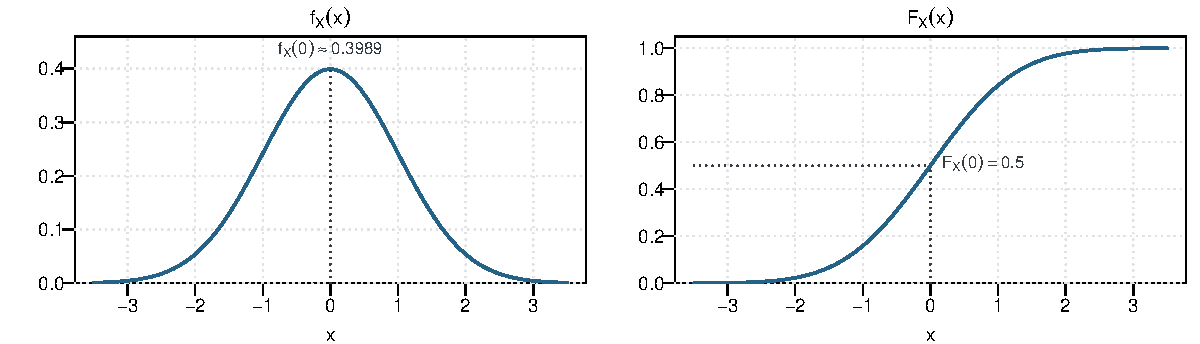
\includegraphics[width=\linewidth]{assets/normal-pdf-cdf.pdf}
\end{center}

Changing the parameters changes the bell in two different ways: $\mu$ moves
it left or right, while $\sigma^2$ stretches it. A small $\sigma^2$ gives a
tall, narrow bell and a steep CDF; a large $\sigma^2$ a low, wide bell and a
CDF that grows slowly.

\begin{center}
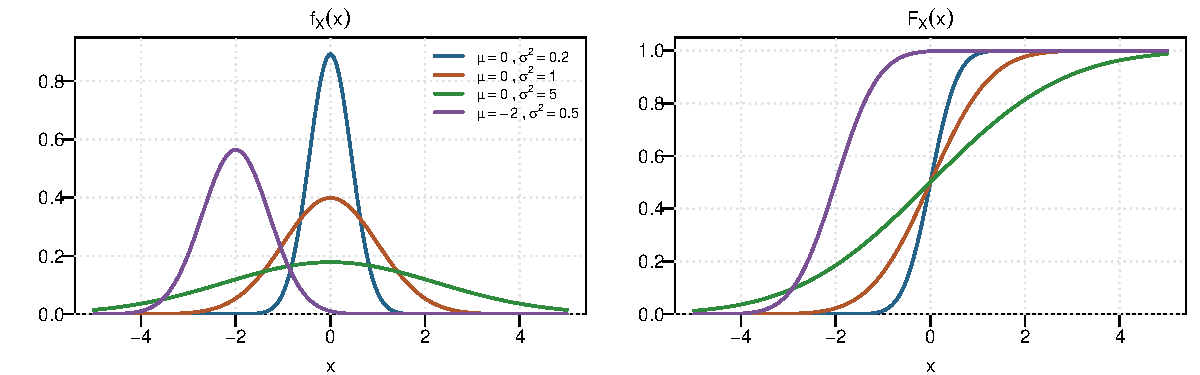
\includegraphics[width=\linewidth]{assets/normal-family.pdf}
\end{center}

\subsection{The standard Normal}

Among all the Normals, one has a special name.

\begin{frameddefn}{Standard Normal}\label{def:standard-normal}
$X$ has a \textbf{standard Normal distribution} if $(\mu,\sigma^2)=(0,1)$.
A standard Normal random variable is traditionally denoted by $Z$, and its
density and CDF by
\[
\phi(z)=\frac{1}{\sqrt{2\pi}}\,e^{-\frac{z^2}{2}},
\qquad
\Phi(z)=\int_{-\infty}^{z}\phi(t)\,\mathrm{d}t,
\qquad z\in\mathbb{R}.
\]
\end{frameddefn}

Why is it so important? Because every Normal can be turned into the
standard one, and vice versa.

\begin{framedprop}{Standardization}\label{prop:standardization}
\begin{enumerate}
\item Any Normal can be turned into the standard Normal.\\[6pt]
If $X\sim N(\mu,\sigma^2)$, then $Z=\dfrac{X-\mu}{\sigma}\sim N(0,1)$.
\item The standard Normal can be turned into any Normal.\\[6pt]
Conversely, if $Z\sim N(0,1)$, then $X=\mu+\sigma Z\sim N(\mu,\sigma^2)$.
\item The quantile of a Normal is obtained by taking the one of the standard
Normal and transforming it like any other value, that is, multiplying by
$\sigma$ and adding $\mu$.\\[6pt]
If $q_p$ and $z_p$ are the quantiles of level $p$ of $N(\mu,\sigma^2)$
and of $N(0,1)$, then $q_p=\mu+z_p\,\sigma$.
\end{enumerate}
\end{framedprop}

\begin{proof}[Proof (point 1)]
To show that $Z\sim N(0,1)$, we go in three steps:
\begin{enumerate}
\item we start from the CDF of $Z$;
\item we differentiate it to get the density $f_Z$;
\item we compare $f_Z$ with $\phi$, which has an explicit formula.
\end{enumerate}
If the densities coincide, so do the CDFs, since the CDF is the integral of
the density.

Since $\sigma>0$, multiplying by $\sigma$ and
adding $\mu$ on both sides keeps the inequality, so
\[
F_Z(z)=P(Z\le z)=P\Big(\frac{X-\mu}{\sigma}\le z\Big)=P(X\le\mu+\sigma z)
=F_X(\mu+\sigma z).
\]
Differentiating with respect to $z$ gives
\[
f_Z(z)=f_X(\mu+\sigma z)\,\sigma .
\]
Finally we evaluate the Normal density at $x=\mu+\sigma z$:
\[
f_Z(z)=\sigma\cdot\frac{1}{\sqrt{2\pi\sigma^2}}\,
e^{-\frac{(\mu+\sigma z-\mu)^2}{2\sigma^2}}
=\sigma\cdot\frac{1}{\sigma\sqrt{2\pi}}\,e^{-\frac{\sigma^2z^2}{2\sigma^2}}
=\frac{1}{\sqrt{2\pi}}\,e^{-\frac{z^2}{2}}=\phi(z),
\]
which is the density of $N(0,1)$.
\end{proof}

\begin{proof}[Proof (point 2)]
To show that $X\sim N(\mu,\sigma^2)$, we go in three steps:
\begin{enumerate}
\item we start from the CDF of $X$;
\item we differentiate it to get the density $f_X$;
\item we compare $f_X$ with the density of the
\hyperref[def:normal]{Normal distribution}, which has an explicit formula.
\end{enumerate}
If the densities coincide, so do the CDFs, since the CDF is the integral of
the density.

Since $\sigma>0$, subtracting $\mu$ and
dividing by $\sigma$ on both sides keeps the inequality, so
\[
F_X(x)=P(X\le x)=P(\mu+\sigma Z\le x)=P\Big(Z\le\frac{x-\mu}{\sigma}\Big)
=\Phi\Big(\frac{x-\mu}{\sigma}\Big).
\]
Differentiating with respect to $x$ gives
\[
f_X(x)=\phi\Big(\frac{x-\mu}{\sigma}\Big)\,\frac{1}{\sigma}.
\]
Finally we evaluate the standard Normal density at $z=(x-\mu)/\sigma$:
\[
f_X(x)=\frac{1}{\sigma}\cdot\frac{1}{\sqrt{2\pi}}\,
e^{-\frac{1}{2}\left(\frac{x-\mu}{\sigma}\right)^2}
=\frac{1}{\sqrt{2\pi\sigma^2}}\,e^{-\frac{(x-\mu)^2}{2\sigma^2}},
\]
which is the density of $N(\mu,\sigma^2)$.
\end{proof}

\begin{proof}[Proof (point 3)]
By point 2, every value $z$ of $Z$ becomes the value $\mu+\sigma z$ of $X$.
Point 3 says that the quantile $z_p$ becomes the quantile $q_p$. Since $q_p$
is, by definition, the point that leaves area $p$ on its left under
$N(\mu,\sigma^2)$, we check that the candidate $\mu+\sigma z_p$ has this
property:
\begin{enumerate}
\item we write $X=\mu+\sigma Z$, by point 2;
\item since $\sigma>0$, subtracting $\mu$ and dividing by $\sigma$ on both
sides keeps the inequality;
\item $z_p$ leaves area $p$ on its left, that is, $\Phi(z_p)=p$.
\end{enumerate}
Then
\[
P(X\le\mu+\sigma z_p)\overset{1}{=}P(\mu+\sigma Z\le\mu+\sigma z_p)
\overset{2}{=}P(Z\le z_p)\overset{3}{=}p ,
\]
so the candidate is the quantile: $q_p=\mu+z_p\,\sigma$.
\end{proof}

\begin{framedexample}{Standardizing the heights}
Let us see an example of the first point of
Proposition~\ref{prop:standardization}.

Let the heights be $X\sim N(170,10^2)$. Standardizing moves the
bell from $170$ to $0$ and shrinks its width from $10$ to $1$.

A student
$190$\,cm tall becomes $z=(190-170)/10=2$: that is, the student lies
$2\sigma=20$\,cm above the centre $\mu$.

\begin{center}
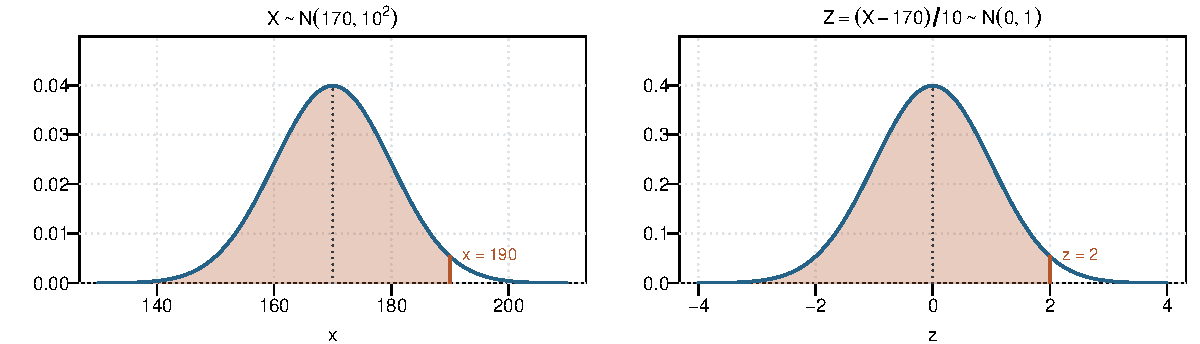
\includegraphics[width=\linewidth]{assets/normal-standardization.pdf}
\end{center}
\end{framedexample}


\begin{studylater}
\subsection{Normal probabilities}

We want to compute $P(a<X<b)$ for any Normal $X\sim N(\mu,\sigma^2)$. But
the CDF of the Normal has no explicit form, so there is no formula to compute
by hand. For the standard Normal, however, the values of $\Phi$ are
tabulated.

The idea is to use point 1 of
Proposition~\ref{prop:standardization}: we bring the probability back to $Z$,
and then use $\Phi$. We go in three steps:
\begin{enumerate}
\item we standardize all three sides, subtracting $\mu$ and dividing by
$\sigma$; since $\sigma>0$, the event does not change;
\item in the middle there is $Z$, since $\frac{X-\mu}{\sigma}=Z\sim N(0,1)$
by point 1;
\item the area between two points is the CDF at the right point minus the CDF
at the left point.
\end{enumerate}
Then
\begin{align*}
P(a<X<b)
&\overset{1}{=}P\Big(\frac{a-\mu}{\sigma}<\frac{X-\mu}{\sigma}<\frac{b-\mu}{\sigma}\Big)
\overset{2}{=}P\Big(\frac{a-\mu}{\sigma}<Z<\frac{b-\mu}{\sigma}\Big)\\
&\overset{3}{=}\Phi\Big(\frac{b-\mu}{\sigma}\Big)-\Phi\Big(\frac{a-\mu}{\sigma}\Big).
\end{align*}
For any Normal it is enough to know $\Phi$: we standardize the endpoints $a$
and $b$, and read $\Phi$ at those two points.

\begin{framedexample}{Normal probabilities}
Let $X\sim N(3,5)$. What is $P(X>1)$? Standardizing,
\begin{align*}
P(X>1)&=1-P(X<1)=1-P\Big(Z<\frac{1-3}{\sqrt5}\Big)=1-\Phi(-0.8944)\\
&=1-\texttt{pnorm(-0.8944)}=0.8144 .
\end{align*}
\end{framedexample}

\subsection{Normal quantiles}

The other way round, we often need the value below which a given probability
lies. Let $Z\sim N(0,1)$ and let $z_p$ be its quantile of level $p$, the
value that solves $p=\Phi(z_p)$. Some quantiles are used so often, in
confidence intervals and statistical tests, that they are worth knowing:
\begin{center}
\begin{tabular}{c|cccccc}
$p$ & $0.9000$ & $0.9500$ & $0.9750$ & $0.9900$ & $0.9950$ & $0.9975$\\
\hline
$z_p$ & $1.28$ & $1.64$ & $1.96$ & $2.33$ & $2.58$ & $2.81$
\end{tabular}
\end{center}
For example, $z_{0.975}\approx1.96$. Since the density $\phi$ is symmetric
around $0$,
\[
z_p=-z_{1-p},
\]
so $-1.96$ leaves $2.5\%$ of the area on its left, and $95\%$ of the area
under $\phi$ lies between $-1.96$ and $1.96$.

\begin{center}
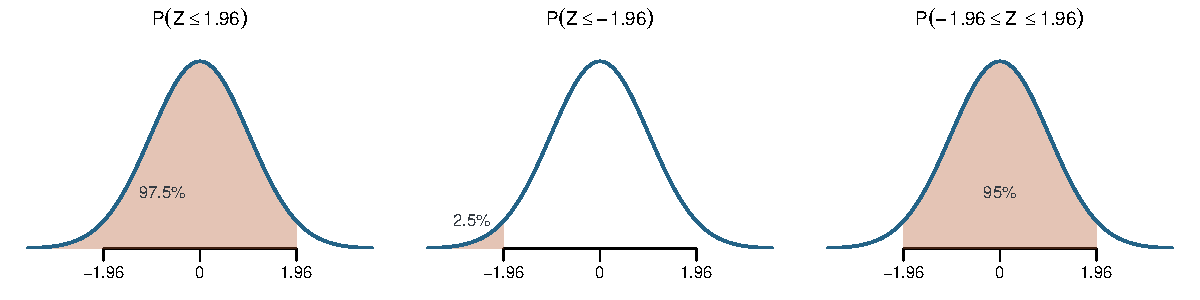
\includegraphics[width=\linewidth]{assets/normal-quantiles.pdf}
\end{center}

More generally, the shortest interval that contains probability $1-\alpha$
is delimited by the quantiles $z_{\alpha/2}$ and $z_{1-\alpha/2}$.

\subsection{Heads-up: light tails}

The Normal is often presented as the most common distribution in the real
world, but it is a special, rather extreme, unimodal distribution. How fast
does its density go to $0$? Up to the constant,
\[
f_X(x)\propto e^{-\frac12x^2}\qquad\text{for } X\sim N(0,1),
\]
so the log-density $-\frac12x^2$ is a parabola: it only decays
quadratically with the distance from the centre. The density itself goes to
$0$ as $e^{-x^2/2}$ when $|x|\to+\infty$, extremely fast, so the probability
of seeing something in the tails is tiny. The Normal has \textbf{light
tails}.

\begin{center}
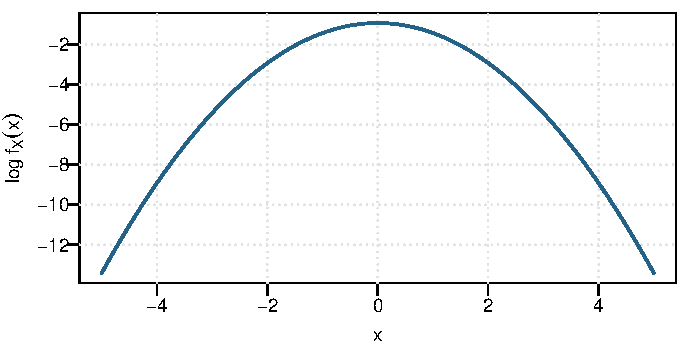
\includegraphics[width=.6\linewidth]{assets/normal-log-density.pdf}
\end{center}

How tiny? The typical deviation of $X$ from the centre $\mu$ is $\sigma$, but
the probabilities that $X$ deviates from $\mu$ by more than $2\sigma$,
$3\sigma$, $4\sigma$ and $5\sigma$ are
\begin{center}
\begin{tabular}{c|cccc}
$k$ & $2$ & $3$ & $4$ & $5$\\
\hline
$P(|X-\mu|>k\sigma)$ & $0.046$ & $0.003$ & $6\cdot10^{-5}$ & $6\cdot10^{-7}$
\end{tabular}
\end{center}
Deviations four or five times larger than the typical one may be rare in a
real population, but not as rare as $6\cdot10^{-5}$. If we model with a
Normal a variable that actually has heavier tails, the rest of the model
will force itself to reduce the deviations of the outliers. The Normal is
too sensitive to outliers, and we need distributions with heavier tails.
\end{studylater}

\section{Student's t distribution}

\begin{frameddefn}{Student's t distribution}\label{def:student-t}
$X$ has a \textbf{Student's $t$ distribution} with $\nu>0$ degrees of
freedom, written $X\sim t_\nu$, if its density is
\[
f_X(x)=\frac{\Gamma\!\big(\frac{\nu+1}{2}\big)}
{\sqrt{\nu\pi}\;\Gamma\!\big(\frac{\nu}{2}\big)}
\Big(1+\frac{x^2}{\nu}\Big)^{-\frac{\nu+1}{2}},\qquad x\in\mathbb{R}.
\]
\end{frameddefn}

\subsection{Cauchy distribution}

With $\nu=1$ the constant becomes
$\Gamma(1)/\big(\sqrt{\pi}\,\Gamma(\tfrac12)\big)=1/\pi$, and the density
takes a particularly simple form.

\begin{frameddefn}{Cauchy distribution}\label{def:cauchy}
$X$ has a \textbf{Cauchy distribution} if its density is
\[
f_X(x)=\frac{1}{\pi\,(x^2+1)},\qquad x\in\mathbb{R},
\]
that is, if $X\sim t_1$.
\end{frameddefn}

\subsubsection{A first look}\label{sec:cauchy-first-look}

The density is symmetric about $0$, because replacing $x$ with $-x$ leaves
$x^2$ unchanged, and it peaks at $f_X(0)=1/\pi\approx0.32$. Its bell shape
resembles the one of the standard Normal (Definition~\ref{def:normal}), but the tails are very different. For large $x$,
$f_X(x)$ behaves like $1/(\pi x^2)$, which decreases only as a power of
$x$, while the standard Normal density decreases like $e^{-x^2/2}$, way faster. At $x=10$ the
Cauchy density is about $0.003$, the standard Normal one about
$8\cdot10^{-23}$. Values far from $0$ are unlikely under the Cauchy, but
not negligible: it has \textbf{heavy tails}.

\begin{center}
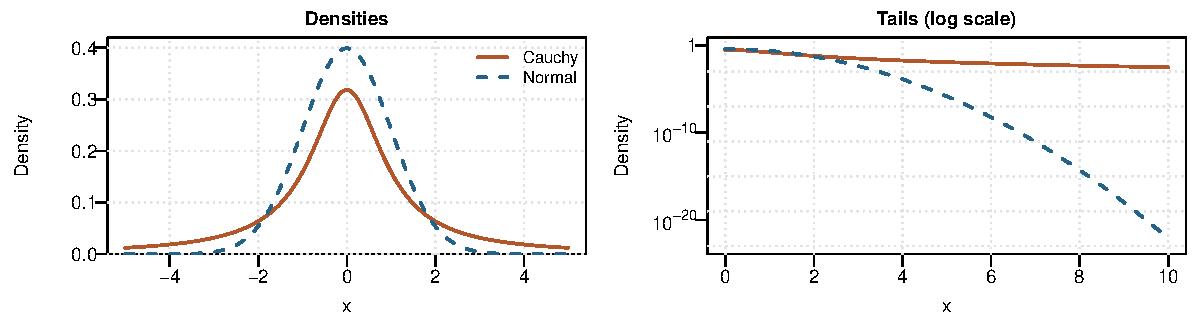
\includegraphics[width=\linewidth]{assets/cauchy-normal.pdf}
\par\smallskip
{\footnotesize Same bell shape near $0$; on a log scale the Normal tail
collapses while the Cauchy tail stays high.}
\end{center}

\subsubsection{Check if \texorpdfstring{$\int_{\mathbb{R}}f_X(x)\,\mathrm{d}x=1$}{the density integrates to 1}}

We need a primitive of $1/(x^2+1)$, and calculus gives one:
\[
\frac{\mathrm{d}}{\mathrm{d}x}\arctan(x)=\frac{1}{x^2+1},\qquad x\in\mathbb{R}.
\]
The arctangent is the inverse of the tangent restricted to
$(-\pi/2,\pi/2)$: the tangent maps that interval onto the whole real line, so
the arctangent maps $\mathbb{R}$ back onto $(-\pi/2,\pi/2)$, with
\[
\lim_{x\to-\infty}\arctan(x)=-\frac{\pi}{2},
\qquad
\lim_{x\to+\infty}\arctan(x)=\frac{\pi}{2}.
\]

\begin{center}
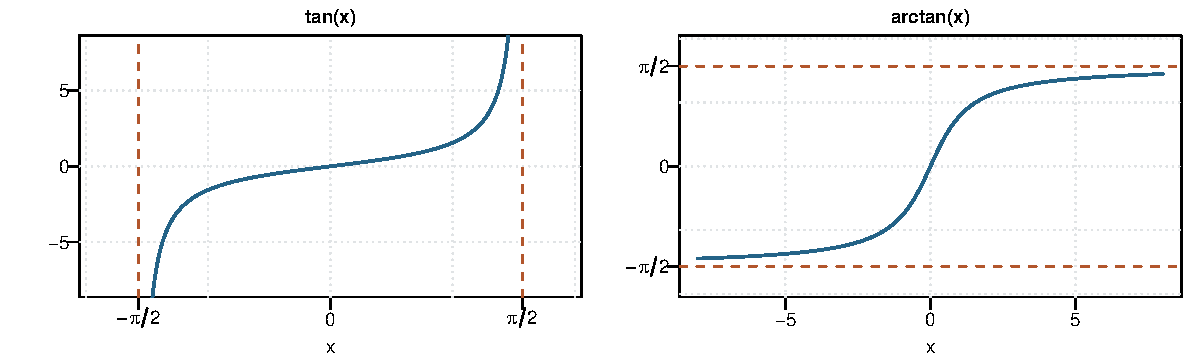
\includegraphics[width=\linewidth]{assets/tan-arctan.pdf}
\end{center}

Hence
\[
\int_{\mathbb{R}}\frac{1}{\pi\,(x^2+1)}\,\mathrm{d}x
=\frac{1}{\pi}\Big[\arctan(x)\Big]_{-\infty}^{+\infty}
=\frac{1}{\pi}\Big(\frac{\pi}{2}-\Big(-\frac{\pi}{2}\Big)\Big)=1 .
\]

\chapter{Learning}

\section{The learning problem}\label{sec:learning}

Why do we collect data? Because we want to understand the process that
produced them. Suppose we want to study the heights of the students of a
university. The heights of all the students have some distribution, with
many values around $170$\,cm and few below $150$ or above $200$. This
distribution, with CDF $F_X$, is the \textbf{population model}: it describes
what varies in the population and how. In a learning problem, however, we do
not know it.

We cannot measure everyone, so we pick $n$ students. Before measuring them,
their heights are random variables $X_1,\ldots,X_n$, where $X_i$ is the
height of the $i$-th student we pick, since we do not know yet who will be
picked. The \textbf{sampling scheme} describes how we pick
them, and the simplest one is IID:
\begin{itemize}
\item \textbf{independent}: the height of the first student tells us nothing
about the height of the second;
\item \textbf{identically distributed}: each $X_i$ has the population
distribution $F_X$, since each student comes from the same population.
\end{itemize}

The population model and the sampling scheme together form the
\textbf{data-generating process}, the machine that produces the numbers we
see. Once we measure, we have the observed data
\[
\mathcal{D}_n=(x_1,\ldots,x_n).
\]
For example, with $n=50$,
\[
\mathcal{D}_{50}=(188,\,164,\,167,\,169,\,165,\,165,\,177,\,171,\,
\ldots,\,169,\,181,\,176,\,173,\,179).
\]
The uppercase $X_i$ is the random variable before measuring; the lowercase
$x_i$ is the number after. In short,
\[
\underbrace{F_X}_{\text{population (unknown)}}
\;\xrightarrow{\text{IID sampling}}\;
\underbrace{X_1,\ldots,X_n}_{\text{random}}
\;\longrightarrow\;
\underbrace{x_1,\ldots,x_n}_{\text{observed data}}.
\]
Probability goes from left to right: if we know $F_X$, we can say which data
will come out.

\textbf{Learning} goes in the other direction: we start from the observed
data and try to recover the population distribution:
\[
\underbrace{F_X}_{\text{?}}\;\longleftarrow\;\underbrace{x_1,\ldots,x_n}_{\text{known}}.
\]
In practice we choose a
\textbf{model}, a family of distributions $p_\theta$ described by a
\textbf{parameter} $\theta$, which may be one number or several. Choosing a
value of $\theta$ chooses one candidate distribution, and learning means
choosing the value that explains the data best.

\begin{framedexample}{Heights as a Normal model}\label{ex:heights-normal}
For the heights we may assume a Normal distribution, without knowing which
one. Recall from Definition~\ref{def:normal} that a Normal is fixed by its
centre $\mu$ and its spread $\sigma$, so
\[
\theta=(\mu,\sigma^2).
\]
Let us take the $n=50$ heights $\mathcal{D}_{50}$ we measured above. The
first plot shows them as a histogram, with a small mark below for each student: they lie between $162$
and $191$\,cm, mostly around $170$--$175$.

Each value of $\theta$ is a different candidate: $\theta=(170,10^2)$ is a
Normal centred at $170$, while $\theta=(150,5^2)$ is centred at $150$ and
narrower. How well does each one approximate the data? We draw it over the
histogram.

\begin{center}
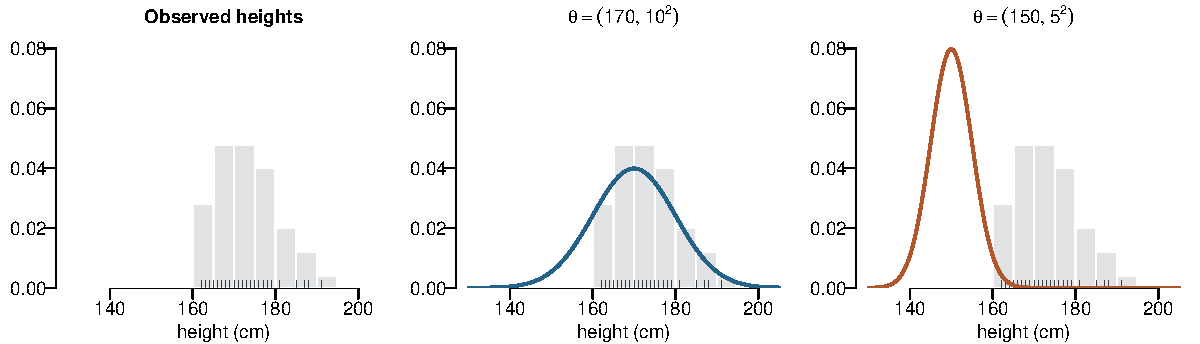
\includegraphics[width=\linewidth]{assets/heights-candidates.pdf}
\end{center}

The first candidate follows the histogram closely. The second puts almost
all its probability below $165$\,cm, where we observed almost no students,
and almost none where most of them are. The first candidate explains the
data much better than the second.
\end{framedexample}

How do we compare the candidates? The likelihood is exactly what we need.

\begin{frameddefn}{Likelihood and maximum likelihood}\label{def:likelihood}
The \textbf{likelihood} of $\theta$ is the joint density of the observed
data, seen as a function of $\theta$. For IID data it is the product
\[
L(\theta)=\prod_{i=1}^n p_\theta(x_i).
\]
The \textbf{maximum likelihood estimate} is the value that makes it largest:
\[
\hat\theta=\arg\max_{\theta}\,L(\theta).
\]
\end{frameddefn}

The likelihood is a product of $n$ factors. Taking the logarithm turns it
into a sum, since $\log(ab)=\log a+\log b$.

\begin{frameddefn}{Log-likelihood}\label{def:log-likelihood}
The \textbf{log-likelihood} is the logarithm of the likelihood. For IID data
it is the sum
\[
\ell(\theta)=\log L(\theta)=\sum_{i=1}^n\log p_\theta(x_i).
\]
\end{frameddefn}

Why is it convenient?
\begin{enumerate}
\item \textbf{Sums are easy to differentiate, products are not.} To find the
maximum we differentiate and set the derivative to $0$. The derivative of a
sum is the sum of the derivatives, while the derivative of a product is
more complex.
\item \textbf{No tiny numbers.} The likelihood multiplies $n$ values that
are often smaller than $1$, so it shrinks quickly as $n$ grows and soon
becomes too small to handle, even for a computer. The log-likelihood adds
their logarithms instead, so it stays an ordinary number.
\end{enumerate}

Why do the likelihood and the log-likelihood have the same maximum? Let
$\hat\theta$ maximise $L$, so that
\[
L(\hat\theta)\ge L(\theta)\qquad\text{for every }\theta .
\]
Since $\log$ is increasing, applying it to both sides keeps the inequality:
\[
\log L(\hat\theta)\ge\log L(\theta),
\]
that is,
\[
\ell(\hat\theta)\ge\ell(\theta)\qquad\text{for every }\theta,
\]
so $\hat\theta$ maximises $\ell$ too. The same argument works backwards, with the exponential,
which is increasing as well. Hence
\[
\hat\theta=\arg\max_{\theta}L(\theta)=\arg\max_{\theta}\ell(\theta):
\]
the values change, the point of maximum does not.

For a Normal model the maximum can be found by hand.

\begin{framedprop}{Maximum likelihood for a Normal}\label{prop:mle-normal}
Let $x_1,\ldots,x_n$ be IID data from $N(\mu,\sigma^2)$. The maximum
likelihood estimates of $\mu$ and $\sigma^2$ are
\[
\hat\mu=\frac1n\sum_{i=1}^n x_i=\bar x,\qquad
\hat\sigma^2=\frac1n\sum_{i=1}^n(x_i-\bar x)^2 .
\]
\end{framedprop}

\begin{proof}
The density of a single observation is
\[
p_\theta(x_i)=\frac{1}{\sqrt{2\pi\sigma^2}}\,e^{-\frac{(x_i-\mu)^2}{2\sigma^2}} .
\]
Its logarithm splits the product into a sum, and undoes the exponential,
since $\log e^{a}=a$:
\[
\log p_\theta(x_i)=\log\frac{1}{\sqrt{2\pi\sigma^2}}-\frac{(x_i-\mu)^2}{2\sigma^2}
=-\frac12\log(2\pi\sigma^2)-\frac{(x_i-\mu)^2}{2\sigma^2},
\]
where we used $\log\frac{1}{\sqrt a}=-\frac12\log a$. The log-likelihood is
the sum over the $n$ observations; the first term is the same for all of
them, so it appears $n$ times:
\[
\ell(\mu,\sigma^2)=-\frac n2\log(2\pi\sigma^2)
-\frac{1}{2\sigma^2}\sum_{i=1}^n(x_i-\mu)^2 .
\]
We set the derivatives to $0$. The first term does not contain $\mu$, so
\[
\frac{\partial\ell}{\partial\mu}=\frac{1}{\sigma^2}\sum_{i=1}^n(x_i-\mu)=0
\quad\Longrightarrow\quad
\hat\mu=\frac1n\sum_{i=1}^n x_i=\bar x ,
\]
since the equation is linear in $\mu$. Then
\[
\frac{\partial\ell}{\partial\sigma^2}=-\frac{n}{2\sigma^2}
+\frac{1}{2\sigma^4}\sum_{i=1}^n(x_i-\mu)^2=0
\quad\Longrightarrow\quad
\hat\sigma^2=\frac1n\sum_{i=1}^n(x_i-\bar x)^2 .
\]
\end{proof}

The best centre is the mean of the data, and the best spread measures how
far the data are from it.

\begin{framedexamplepart}{ex:heights-normal}{2}{Heights as a Normal model}\label{ex:heights-likelihood}
Let us take the heights of Example~\ref{ex:heights-normal} again. From the
plots, the first candidate explains the data much better than the second. Does the likelihood say the same?

First we evaluate each density at every observed value:
\begin{center}
\begin{tabular}{c|cc}
$x_i$ & $\theta=(170,10^2)$ & $\theta=(150,5^2)$\\
\hline
$188$ & $0.0079$ & $2\cdot10^{-14}$\\
$164$ & $0.033$ & $0.0016$\\
$167$ & $0.038$ & $0.00025$\\
$\vdots$ & $\vdots$ & $\vdots$
\end{tabular}
\end{center}

Then we multiply the $50$ values:
\[
L(170,10^2)\approx2\cdot10^{-77},\qquad L(150,5^2)\approx9\cdot10^{-319}.
\]
Both numbers are tiny, since we multiply $50$ values smaller than $1$; what
matters is the comparison:
\[
\frac{L(170,10^2)}{L(150,5^2)}\approx10^{241}.
\]
The likelihood agrees with the plots.

Maximum likelihood looks for the
largest $L$ among all the candidates, not only these two. By
Proposition~\ref{prop:mle-normal}, for these data it is reached at
$\hat\theta=(\bar x,\hat\sigma^2)\approx(173.6,\,7.0^2)$, with
$L(\hat\theta)\approx9\cdot10^{-74}$.
\end{framedexamplepart}

Summing up, learning goes in four steps.

\begin{framedalgo}{Learning a model from data}\label{alg:learning}
\begin{enumerate}
\item \textbf{Data.} Collect IID data $\mathcal{D}_n=(x_1,\ldots,x_n)$.
\item \textbf{Model.} Choose a family of distributions $p_\theta$, with
parameter $\theta$.
\item \textbf{Likelihood.} Write the likelihood of the data,
$L(\theta)=\prod_{i=1}^n p_\theta(x_i)$.
\item \textbf{Maximum likelihood.} Choose
$\hat\theta=\arg\max_{\theta}L(\theta)$, or equivalently
$\arg\max_{\theta}\ell(\theta)$.
\end{enumerate}
\end{framedalgo}

Example~\ref{ex:heights-normal} and its part~2 follow
exactly these steps:
\begin{enumerate}
\item \textbf{Data:} the $n=50$ heights $\mathcal{D}_{50}$;
\item \textbf{Model:} a Normal, with $\theta=(\mu,\sigma^2)$;
\item \textbf{Likelihood:} the product of the Normal densities at the $50$
heights;
\item \textbf{Maximum likelihood:} $\hat\theta\approx(173.6,\,7.0^2)$.
\end{enumerate}

\section{Hidden variables and mixtures}\label{sec:hidden}

In Section~\ref{sec:learning} each observation $x_i$ was a height, and the
model $p_\theta$ described the heights directly. Often, however, behind what
we observe, like an image, a symbol or an audio recording, there is something
we do not see, which affects what we see: a \textbf{hidden} variable.

For example, we measure the height of a person without knowing whether the
person is a man or a woman. The sex matters, since men are taller on
average, but we do not observe it. Then
\begin{itemize}
\item $\text{obs}$ is the height, what we see;
\item $\text{hid}$ is the sex, what is hidden.
\end{itemize}

We describe the two together with a joint distribution
$p(\text{obs},\text{hid})$. By the product rule it splits into two pieces:
\[
\begin{bmatrix}\text{obs}\\ \text{hid}\end{bmatrix}\sim
\underbrace{p(\text{obs},\text{hid})}_{\text{joint}}
=\underbrace{p(\text{obs}\mid\text{hid})}_{\text{conditional}}\,
\underbrace{p(\text{hid})}_{\text{marginal}}.
\]
We can read it as a story in two steps: first the hidden value is drawn with
probability $p(\text{hid})$, then, given that value, the observation is
drawn from $p(\text{obs}\mid\text{hid})$.

What is the distribution of what we actually see? We do not know the hidden
value, so we integrate it out over its support $\operatorname{supp}(\text{hid})$, the
set of all the values it can take:
\[
p(\text{obs})=\int_{\operatorname{supp}(\text{hid})} p(\text{obs},\text{hid})\,\mathrm{d}\,\text{hid}.
\]

\begin{framedexample}{Heights of men and women}\label{ex:men-women}
In the height example the support of the hidden variable is
$\operatorname{supp}(\text{hid})=\{\text{man},\text{woman}\}$, only two values, so the integral
is a sum over the two groups:
\[
p(\text{height})=p(\text{height}\mid\text{man})\,p(\text{man})
+p(\text{height}\mid\text{woman})\,p(\text{woman}).
\]
\end{framedexample}

So $p(\text{obs})$ is a weighted average of several distributions, one for
each hidden value, weighted by how likely that value is: it is a
\textbf{mixture}.

\begin{framedexamplepart}{ex:men-women}{2}{Heights of men and women}
Let us take the heights of Example~\ref{ex:men-women} again, where
$p(\text{height})$ is a sum over the two groups. Why is it a weighted
average of distributions? Let us label each piece:
\[
p(\text{height})=
\underbrace{p(\text{height}\mid\text{man})}_{\text{distribution of the men}}
\cdot\underbrace{p(\text{man})}_{\text{weight}}
+\underbrace{p(\text{height}\mid\text{woman})}_{\text{distribution of the women}}
\cdot\underbrace{p(\text{woman})}_{\text{weight}}.
\]
For each hidden value there is a distribution of the heights: a bell for the
men and one for the women. Each bell is multiplied by the probability of its
group, and the weights add up to $p(\text{man})+p(\text{woman})=1$. So
$p(\text{height})$ is a weighted average of the two bells.

In the plot below the two groups have the same weight,
$p(\text{man})=p(\text{woman})=0.5$.

\begin{center}
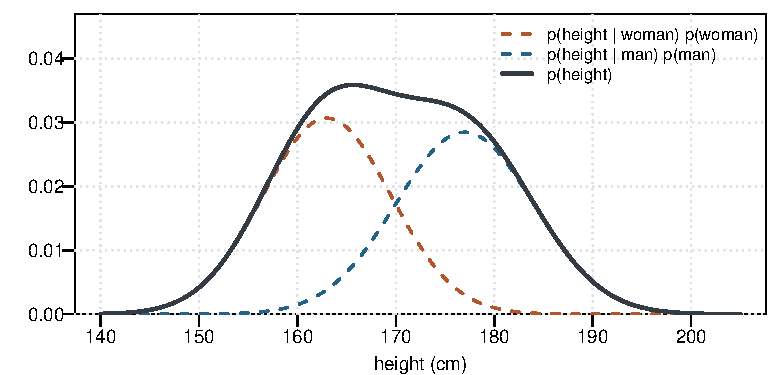
\includegraphics[width=.75\linewidth]{assets/heights-mixture.pdf}
\end{center}
\end{framedexamplepart}

\subsection{Finite mixtures}\label{sec:finite-mixtures}

In Example~\ref{ex:men-women} the hidden variable had only two values, man
and woman. What happens if the population is made of $K$ groups instead of
two?

We make two assumptions:
\begin{enumerate}
\item The hidden variable $\text{hid}$ has a finite support,
$\operatorname{supp}(\text{hid})=\{1,\ldots,K\}$: each value is a group, or
\textbf{sub-population}. The probability of each group is, again, a
\textbf{weight},
\[
\pi_k=P(\text{hid}=k),\qquad k=1,\ldots,K.
\]
The weights are probabilities, so they are non-negative and add up to $1$.
Vectors like this have a name.

\begin{frameddefn}{Simplex}\label{def:simplex}
The \textbf{simplex} of dimension $K-1$ is the set
\[
\Delta^{K-1}=\Big\{(p_1,\ldots,p_K)\in\mathbb{R}^K\ \Big|\ p_i\ge0,\
\sum_{i=1}^K p_i=1\Big\}.
\]
\end{frameddefn}

So the vector of weights lies in the simplex:
$(\pi_1,\ldots,\pi_K)\in\Delta^{K-1}$.
\item Inside each group the observation has its own distribution, usually
from a simple family:
\[
(\text{obs}\mid \text{hid}=k)\sim f_k(o).
\]
It may be discrete or continuous, univariate or multivariate.
\end{enumerate}

We are still interested in computing the distribution of what we actually
see. As in Section~\ref{sec:hidden}, we sum out the hidden variable:
\[
f_{\text{obs}}(o)=\int_{\operatorname{supp}(\text{hid})}p(o,\,h)\,\mathrm{d}h .
\]
Since $\text{hid}$ takes only the values $1,\ldots,K$, the integral becomes a sum:
\[
f_{\text{obs}}(o)=\sum_{k=1}^K p(o,\,\text{hid}=k).
\]
Each term splits, by the multiplication rule, into a conditional and a
marginal:
\[
p(o,\,\text{hid}=k)=\underbrace{p(o\mid \text{hid}=k)}_{f_k(o)\text{ (assumption 2)}}\cdot
\underbrace{P(\text{hid}=k)}_{\pi_k\text{ (assumption 1)}}.
\]
Since we know both pieces on the right-hand side from the two assumptions, putting them together
gives the following model.

\begin{frameddefn}{Finite mixture model}\label{def:finite-mixture}
A \textbf{finite mixture model} with $K$ \textbf{components} has density (or
mass function)
\[
f_{\text{obs}}(o)=\sum_{j=1}^K f_j(o)\,\pi_j,
\]
where $f_1,\ldots,f_K$ are the distributions of the $K$ groups and
$(\pi_1,\ldots,\pi_K)\in\Delta^{K-1}$ are their weights.
\end{frameddefn}

\begin{framedexamplepart}{ex:men-women}{3}{Heights of men and women}\label{ex:men-women-3}
Let us take the heights of Example~\ref{ex:men-women} again, where
\[
p(\text{height})=p(\text{height}\mid\text{man})\,p(\text{man})
+p(\text{height}\mid\text{woman})\,p(\text{woman}).
\]
Is it a finite mixture? Yes, with $K=2$ groups: the hidden variable $\text{hid}$
takes the values woman and man, with weights and distributions
\[
\pi_1=p(\text{woman}),\quad \pi_2=p(\text{man}),\qquad
f_1=p(\text{height}\mid\text{woman}),\quad f_2=p(\text{height}\mid\text{man}).
\]
\end{framedexamplepart}

\subsubsection{Gaussian mixtures}\label{sec:gmm}

The finite mixture leaves the distribution $f_k$ of each group free: it can
be anything. The most common choice is a Normal in every group, each with
its own centre $\mu_j$ and its own spread $\sigma_j$:
\[
f_j(o)=N(o\mid\mu_j,\sigma_j^2),\qquad j=1,\ldots,K.
\]

\begin{frameddefn}{Gaussian mixture model}\label{def:gmm}
A \textbf{Gaussian mixture model} (GMM) with $K$ components has density
\[
f_{\text{obs}}(o)=\sum_{j=1}^K\pi_j\,N(o\mid\mu_j,\sigma_j^2),
\]
with parameters
$\theta=\{\pi_j,\,\mu_j,\,\sigma_j^2\}_{j=1}^K$, where
$(\pi_1,\ldots,\pi_K)\in\Delta^{K-1}$.
\end{frameddefn}

A single Normal always has one bump and is symmetric. By adding $K$ weighted
bells we can describe data with several bumps, or asymmetric ones. For
example, with $K=3$:

\begin{center}
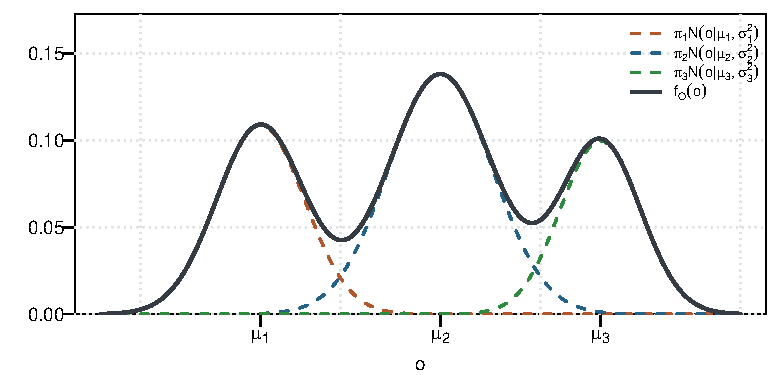
\includegraphics[width=.75\linewidth]{assets/gmm-three.pdf}
\end{center}

\begin{framedexamplepart}{ex:men-women}{4}{Heights of men and women}\label{ex:men-women-4}
Let us take the heights of Example~\ref{ex:men-women} part~3 again: a finite
mixture with $K=2$ groups, women and men, with weights $\pi_1,\pi_2$ and
distributions $f_1=p(\text{height}\mid\text{woman})$,
$f_2=p(\text{height}\mid\text{man})$. Is it a Gaussian mixture?

It is, if the heights inside each group are Normal:
\[
f_1=N(\mu_1,\sigma_1^2),\qquad f_2=N(\mu_2,\sigma_2^2).
\]
Then
\[
p(\text{height})=\pi_1\,N(\text{height}\mid\mu_1,\sigma_1^2)
+\pi_2\,N(\text{height}\mid\mu_2,\sigma_2^2),
\]
a GMM with $K=2$ and parameters
$\theta=\{\pi_1,\pi_2,\mu_1,\mu_2,\sigma_1^2,\sigma_2^2\}$.
\end{framedexamplepart}

How do we learn the $\theta$ of a GMM from data? Let us follow the steps of
Algorithm~\ref{alg:learning}, writing the data as $o_1,\ldots,o_n$, the observed
values of $\text{obs}$:
\begin{enumerate}
\item \textbf{Data:} IID observations $o_1,\ldots,o_n$;
\item \textbf{Model:} the GMM of Definition~\ref{def:gmm}, with
$\theta=\{\pi_j,\mu_j,\sigma_j^2\}_{j=1}^K$;
\item \textbf{Likelihood:} as always $L(\theta)=\prod_{i=1}^n p_\theta(o_i)$,
but now each factor is the density of the GMM,
\[
p_\theta(o_i)=\sum_{j=1}^K\pi_j\,N(o_i\mid\mu_j,\sigma_j^2),
\]
so that
\[
L(\theta)=\prod_{i=1}^n\ \sum_{j=1}^K\pi_j\,N(o_i\mid\mu_j,\sigma_j^2);
\]
\item \textbf{Maximum likelihood:} $\hat\theta=\arg\max_{\theta}L(\theta)$.
\end{enumerate}
Steps 1, 2 and 3 work as before. Step 4 is where we get stuck. Why?

To see why, consider first the case where we know the group of every
observation: its hidden label $\text{hid}_i$ takes an observed value $h_i$.

\begin{framedprop}{Maximum likelihood for a GMM with labels}\label{prop:mle-gmm-labels}
Let $o_1,\ldots,o_n$ be IID data from a GMM with $K$ components, and suppose
that the group $h_i$ of every observation is known. Let $n_j$ be the number
of observations in group $j$. Then the maximum likelihood estimates are
\[
\hat\pi_j=\frac{n_j}{n},\qquad
\hat\mu_j=\frac{1}{n_j}\sum_{i:\,h_i=j}o_i,\qquad
\hat\sigma_j^2=\frac{1}{n_j}\sum_{i:\,h_i=j}(o_i-\hat\mu_j)^2,
\qquad j=1,\ldots,K.
\]
\end{framedprop}

\begin{proof}
Recall that, without labels, the likelihood of a GMM is
\[
L(\theta)=\prod_{i=1}^n\ \sum_{j=1}^K\pi_j\,N(o_i\mid\mu_j,\sigma_j^2).
\]
With the labels we know that it is $h_i$, so only the term
$j=h_i$ of the sum remains:
\[
L(\theta)=\prod_{i=1}^n\pi_{h_i}\,N(o_i\mid\mu_{h_i},\sigma_{h_i}^2).
\]
Taking the logarithm, the product over $i$ becomes a sum, and each factor
splits since $\log(ab)=\log a+\log b$:
\[
\ell(\theta)=\sum_{i=1}^n\Big[\log\pi_{h_i}+\log N(o_i\mid\mu_{h_i},\sigma_{h_i}^2)\Big].
\]
Grouping the terms by group, it breaks into separate pieces:
\[
\ell(\theta)=\underbrace{\sum_{j=1}^K n_j\log\pi_j}_{\text{only the weights}}
+\sum_{j=1}^K\ \underbrace{\sum_{i:\,h_i=j}\log N(o_i\mid\mu_j,\sigma_j^2)}_{\text{only }\mu_j\text{ and }\sigma_j^2}.
\]
The parameters $\mu_j$ and $\sigma_j^2$ appear only in the $j$-th inner sum,
which is the log-likelihood of a single Normal on the $n_j$ observations of
group $j$. By Proposition~\ref{prop:mle-normal}, its maximum is at the mean
and the spread of the group. The weights appear only in the first sum;
maximising it under the constraint $\sum_j\pi_j=1$ gives, as one can show,
$\hat\pi_j=n_j/n$.
\end{proof}


\begin{framedexamplepart}{ex:men-women}{5}{Heights of men and women}
Let us take the heights of Example~\ref{ex:men-women} part~4 again: a GMM with
$K=2$ groups, women and men. Can we learn its $\theta$ following Algorithm~\ref{alg:learning}?

\withlabels\par\smallskip
Suppose first that we measured $50$ people and recorded, next to each
height, also the group:
\begin{center}
\begin{tabular}{c|c}
height & group\\
\hline
$147$ & woman\\
$166$ & woman\\
$182$ & man\\
$184$ & man\\
$167$ & man\\
$\vdots$ & $\vdots$
\end{tabular}
\end{center}
Then learning would be easy: we are in the case of
Proposition~\ref{prop:mle-gmm-labels}, with $K=2$, $n_1=25$ women and
$n_2=25$ men. In practice we split the data in two and on each part we learn
a single Normal, exactly as we did for all the heights in
Example~\ref{ex:heights-normal} and its part~2. For these data,
\[
\hat\theta_{\text{women}}\approx(160.5,\,7.1^2),\qquad
\hat\theta_{\text{men}}\approx(176.3,\,7.4^2),
\]
and each fitted Normal follows its own histogram:

\begin{center}
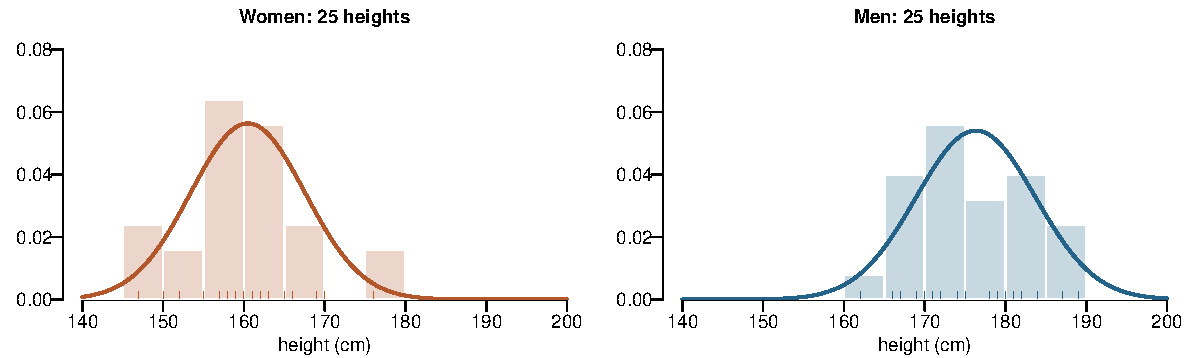
\includegraphics[width=\linewidth]{assets/heights-split.pdf}
\end{center}

The weights are the fractions of each group:
\[
\hat\pi_1=\frac{n_1}{n}=\frac{25}{50}=0.5,\qquad
\hat\pi_2=\frac{n_2}{n}=\frac{25}{50}=0.5.
\]

\withoutlabels\par\smallskip
In practice, however, the column ``group'' is missing: we only see the
heights. So every factor of the likelihood is the sum of the two bells:
\[
L(\theta)=\prod_{i=1}^n\Big[\pi_1\,N(o_i\mid\mu_1,\sigma_1^2)
+\pi_2\,N(o_i\mid\mu_2,\sigma_2^2)\Big].
\]
The log-likelihood of Definition~\ref{def:log-likelihood} still turns the
product into a sum, but inside each term a logarithm of a sum remains:
\[
\ell(\theta)=\sum_{i=1}^n\log\Big(\pi_1\,N(o_i\mid\mu_1,\sigma_1^2)
+\pi_2\,N(o_i\mid\mu_2,\sigma_2^2)\Big).
\]
This is where we get stuck: $\log(a+b)\neq\log a+\log b$, so the parameters
of the women and of the men stay tangled together in every term, and they no
longer separate.

What happens if we set a derivative to $0$ anyway? For $\mu_1$,
\[
\frac{\partial\ell}{\partial\mu_1}=\sum_{i=1}^n
\frac{\pi_1N(o_i\mid\mu_1,\sigma_1^2)}
{\pi_1N(o_i\mid\mu_1,\sigma_1^2)+\pi_2N(o_i\mid\mu_2,\sigma_2^2)}\,
\frac{o_i-\mu_1}{\sigma_1^2}=0 .
\]
Here $\mu_1$ appears both in $o_i-\mu_1$ and inside the exponentials of the
Normal densities, in the numerator and in the denominator. Unlike the linear
equation of Proposition~\ref{prop:mle-normal}, no algebraic step isolates $\mu_1$:
there is no formula for $\hat\theta$. The maximum still exists, but we can
only approach it step by step.
\end{framedexamplepart}

To fit each group we would need to know which observations belong to it,
and to know that we would already need the parameters.

\begin{importantbox}
\phantomsection\label{box:spade}
\textbf{Important.} With the tools we have so far, we cannot compute the
maximum likelihood estimate of a GMM without labels. Later, once we know
more powerful tools, we will be able to solve this problem, which we call
($\spadesuit$).
\end{importantbox}

\chapter{Expected value}

\section{Why summarise a distribution?}

The distribution of a random variable $X$ tells us which values $X$ can
take and how likely each of them is. It contains \emph{all} the
probabilistic information about $X$: once we know it, we can answer any
question such as ``what is the probability that a light bulb lasts more
than 1000 hours?'' or ``that it lasts between 500 and 800 hours?''.

That completeness has a price. As we already know, the distribution is a
\emph{function}: the
probability mass function $p_X(x)$ if $X$ is discrete, the density
$f_X(x)$ if it is continuous, or the cumulative distribution function
$F_X(x)$ in either case. It assigns a value to every possible $x$, often to
infinitely many of them. If we ask ``roughly how long does this bulb last?''
and receive a whole density curve, we have all the information but no
answer. Can we describe $X$ with a few numbers instead of a whole function,
accepting that we lose some information?

\subsection{Median and quantiles}

The simplest \emph{summaries} pick a few points of the distribution and
give up describing the entire curve. We have already met them with the
quantile function, so we only recall them quickly.

The \textbf{median} is the value that splits the distribution in half: $X$
falls below it with probability $1/2$ and above it with probability $1/2$.
If the median lifetime of a bulb is 900 hours, half of the bulbs fail before
900 hours and half after.

The \textbf{quantile} of order $p$ extends the idea to any proportion: it is
the value below which $X$ falls with probability $p$, that is the point
where $F_X$ reaches $p$. The quantile of order $0.5$ is the median, while
the quantiles of order $0.25$ and $0.75$ are the first and third quartiles.
If the quartiles of the bulb lifetime are 600 and 1200 hours, the central
half of the bulbs lasts between 600 and 1200 hours, so three numbers
already describe both the centre and the spread.

They remain summaries, though: two very different distributions, one with
very long tails and one without, can share the same median and quartiles.

\subsection{The expected value as a weighted average}

There is another way to condense $X$ into a single number, which uses \emph{all} its values
at once.

\begin{frameddefn}{Expected value: the intuitive idea}
The \textbf{expectation}, \textbf{expected value} or \textbf{mean}
$\mathbb{E}(X)$ is the weighted average of the possible values of $X$, with
weights equal to their probabilities:
\[
\mathbb{E}(X)=\sum_x x\cdot P(X=x).
\]
\end{frameddefn}

\begin{framedexample}{A fair die}
Each value $1,\ldots,6$ has probability $1/6$, so
\[
\mathbb{E}(X)=1\cdot\tfrac16+2\cdot\tfrac16+\cdots+6\cdot\tfrac16=3.5 .
\]
With equal weights we get the ordinary average. The result shows two
things:
\begin{enumerate}
\item $3.5$ is not a value the die can show, so the expected value is not
``the value we expect to see'';
\item it is rather the \emph{centre} around which the values spread:
averaging a very large number of rolls gives about $3.5$.
\end{enumerate}
\end{framedexample}

\begin{framedexample}{A lottery}\label{ex:lottery}
A ticket wins 10\,\texteuro{} with probability $0.1$ and nothing with
probability $0.9$:
\[
\mathbb{E}(X)=10\cdot0.1+0\cdot0.9=1\text{\,\texteuro}.
\]
The plain average of the two values, $(10+0)/2=5$\,\texteuro, would ignore that
winning is rare. Playing many times, we win 1\,\texteuro{} per game on average,
so a ticket costing more than 1\,\texteuro{} loses money in the long run.
\end{framedexample}

Using the expected value to decide whether a deal pays off is exactly what
the next example does.

\begin{framedexample}{A fair price for a stock}
You have 18\,\texteuro{} and consider buying a share that costs 18\,\texteuro{} and
holding it for one year. After one year the share is worth
\[
\text{Value}=18+X,
\]
where $X$ is the change of the price over the year. The alternative is the
bank at 5\% interest, which returns $18\cdot1.05=18.90$\,\texteuro{} for sure,
a certain gain of $0.90$\,\texteuro.

Today $X$ is unknown: it is a random variable, and a sure number cannot be
compared with a random quantity. We need a \emph{reference value} for $X$, a
single number representing it, which is the summary problem we started
from.

The summary we choose is the gain we ``expect'', $\mathbb{E}(X)$: if
$\mathbb{E}(X)>0.90$\,\texteuro{} the share pays more than the bank on average,
otherwise the bank does.

To see it with numbers, suppose that the price change has distribution
\begin{center}
\begin{tabular}{@{}lcccc@{}}
\toprule
$x$ (\texteuro) & $-2$ & $0$ & $1$ & $3$\\
$P(X=x)$ & $0.1$ & $0.4$ & $0.3$ & $0.2$\\
\bottomrule
\end{tabular}
\end{center}
Then
$\mathbb{E}(X)=(-2)(0.1)+0(0.4)+1(0.3)+3(0.2)=0.70$\,\texteuro, less than
$0.90$\,\texteuro: on average the bank pays more. The 20\% chance of gaining
3\,\texteuro{} is weighed together with the chance of losing and of gaining
nothing.

The \textbf{fair price} $p$ of the share is the one at which share and bank
pay the same on average. Here the share is worth $18.70$\,\texteuro{} on average
after one year, so
\[
\underbrace{p\cdot1.05}_{\substack{\text{$p$ in the bank}\\\text{after one year}}}
=\underbrace{18.70}_{\substack{\text{the share on average}\\\text{after one year}}}
\]
gives $p\approx17.81$\,\texteuro: at 18\,\texteuro{} the share is slightly
overpriced.
\end{framedexample}

The expected value looks only at the average and ignores the \emph{risk}:
the bank gives $0.90$\,\texteuro{} for sure, while the share may lose
2\,\texteuro. Measuring how far $X$ strays from $\mathbb{E}(X)$ will need another
concept called the variance.

\section{The definition}

The intuitive idea becomes precise once we say what ``weight'' means for
discrete and for continuous variables.

\begin{frameddefn}{Expected value}\label{def:expected-value}
The \textbf{expected value} (expectation, mean, first moment) of
$X\sim F_X$ is
\[
\mathbb{E}(X)=
\begin{cases}
\displaystyle\sum_x x\,p_X(x) & \text{if $X$ is discrete with PMF $p_X$,}\\[2ex]
\displaystyle\int_{\mathbb{R}} x\,f_X(x)\,\mathrm{d}x & \text{if $X$ is continuous with PDF $f_X$,}
\end{cases}
\]
provided the sum or the integral is well defined, that is
$\sum_x|x|\,p_X(x)<\infty$ or $\int_{\mathbb{R}}|x|\,f_X(x)\,\mathrm{d}x<\infty$.
\par\medskip\noindent Both cases can be written at once as
\[
\mathbb{E}(X)=\int_{\mathbb{R}}x\,\mathrm{d}F_X(x),
\]
where $\mathrm{d}F_X(x)$ stands for $f_X(x)\,\mathrm{d}x$ in the continuous
case, and the integral becomes the sum $\sum_x x\,p_X(x)$ in the discrete
case.
\end{frameddefn}

What goes in, and what comes out? In goes the whole distribution $F_X$,
which is a function; out comes a single number. A map that takes a function
and returns a number is called a \phantomsection\label{functional}\textbf{functional}, so we
can write
\[
\mathbb{E}(X)=g(F_X),\qquad g\text{ a functional.}
\]

The definition also calls the expected value the \emph{first moment}.
What are the other moments?

\begin{frameddefn}{Moments}\label{def:moments}
For $k=1,2,3,\ldots$, the \textbf{$k$-th moment} of $X$ is the expected
value of its $k$-th power, $\mathbb{E}(X^k)$, provided it exists. The
expected value $\mathbb{E}(X)$ is the first moment.
\end{frameddefn}

\begin{framedexample}{The uniform distribution on $[0,1]$}
Here $f_X(x)=1$ on $[0,1]$, so
\[
\mathbb{E}(X)=\int_0^1 x\cdot1\,\mathrm{d}x=\Big[\tfrac{x^2}{2}\Big]_0^1=\tfrac12,
\]
the centre of the interval, as expected from a distribution that favours
no value.
\end{framedexample}

\section{Property 0: distribution specific}

The name ``expectation \emph{of $X$}'' suggests that $\mathbb{E}(X)$
depends on the random variable in every detail. Recall that $X$ is a
function attaching a number to each outcome of the experiment. The formula,
however, uses only the values $x$ and their probabilities $p_X(x)$, which
is the distribution of $X$. It never asks \emph{which outcome} produces
which value.

\begin{framedprop}{Distribution specific}
$\mathbb{E}(X)$ depends only on the distribution of $X$: two random
variables with the same distribution have the same expected value.
\end{framedprop}

\begin{framedexample}{Heads and tails}
Toss a fair coin once and let $X=1$ if it lands heads and $0$ otherwise,
$Y=1$ if it lands tails and $0$ otherwise. $X$ and $Y$ are never equal:
when one is $1$ the other is $0$. Their tables of values and probabilities,
however, are identical:
\begin{center}
\begin{tabular}{@{}lcc@{}}
\toprule
value & $0$ & $1$\\
probability & $1/2$ & $1/2$\\
\bottomrule
\end{tabular}
\end{center}
so both are Bernoulli$(1/2)$ and $\mathbb{E}(X)=\mathbb{E}(Y)=1/2$. The
expected value cannot tell them apart, because it only sees the
distribution.
\end{framedexample}

\section{Property 1: centre of mass}

The expected value has a physical meaning: it is the point where the
distribution balances.

\subsection{Discrete case: a rod with weights}

Picture the $x$-axis as a rigid, weightless rod, and hang a weight
$p_X(x_j)$ at each value $x_j$. Resting the rod on a support placed at
$\mathbb{E}(X)$, the rod stays level.

\begin{center}
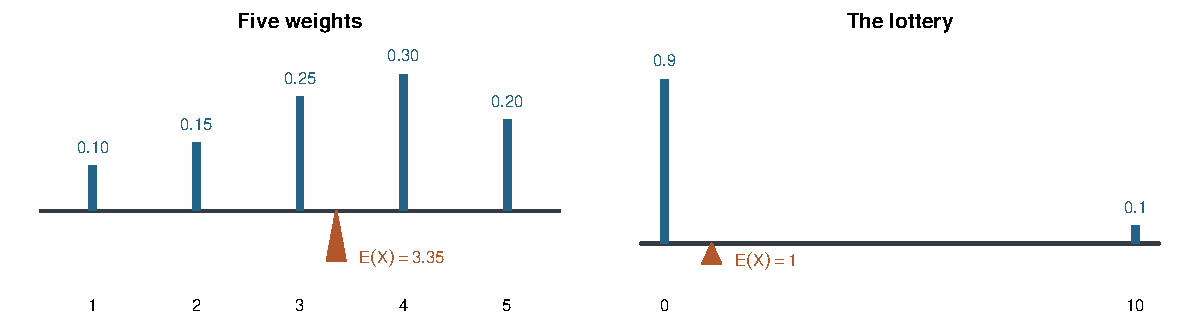
\includegraphics[width=\linewidth]{assets/rod-discrete.pdf}
\par\smallskip
{\footnotesize The support (triangle) at $\mathbb{E}(X)$ balances the rod.}
\end{center}

Why exactly there? A weight on a rod makes the rod turn around the support,
and its turning effect, the \emph{moment}, grows with how heavy the weight
is and how far it hangs from the support, as with a lever. With the support
at $c$, a weight $p$ at $x$ has moment $(x-c)\,p$: positive if it hangs to
the right and pushes the rod to the right, negative if it hangs to the left.
The rod balances when the pushes cancel out:
\[
\sum_j (x_j-c)\,p_X(x_j)=0.
\]
Expanding the sum and using $\sum_j p_X(x_j)=1$ gives
$\mathbb{E}(X)-c=0$, so the support must sit at $c=\mathbb{E}(X)$.

\begin{framedexample}{The lottery as a rod}\label{ex:lottery-rod}
Let us take the lottery of Example~\ref{ex:lottery} again: $X=0$ with
probability $0.9$ and $X=10$ with probability $0.1$, so $\mathbb{E}(X)=1$. As a
rod, it is a weight $0.9$ hanging at $0$ and a weight $0.1$ hanging at $10$.
Does the rod really balance at $1$?

With the support at $c=1$,
\[(0-\underbrace{1}_{c})(0.9)+(10-\underbrace{1}_{c})(0.1)=-0.9+0.9=0,\]
so the rod balances.

With the support at $c=0.5$,
\[(0-\underbrace{0.5}_{c})(0.9)+(10-\underbrace{0.5}_{c})(0.1)=-0.45+0.95=0.5>0,\]
so the rod tips to the right.

\begin{center}
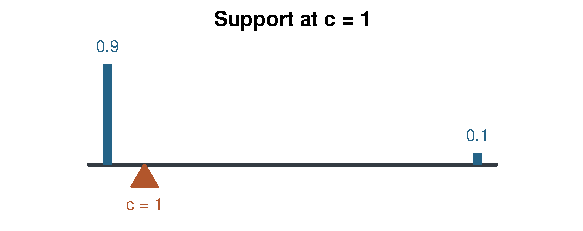
\includegraphics[width=.47\linewidth]{assets/rod-balanced.pdf}\hfill
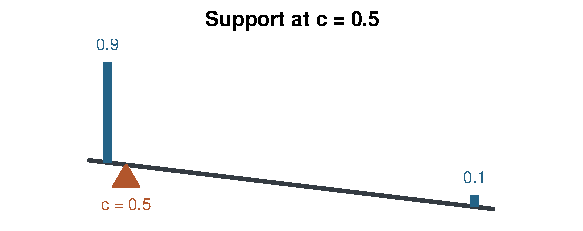
\includegraphics[width=.47\linewidth]{assets/rod-tilted.pdf}
\end{center}
 The small weight is far
away, and its long lever moves the balance point from $0$ to $1$.
\end{framedexample}


\subsection{Continuous case: a rod with spread mass}

When $X$ is continuous no single point carries a weight; the mass is spread
along the rod, like a metal bar that is thicker in some places than in
others. Take the density $f_X(x)$ as the mass per unit length: where the
curve is high the rod is thick and heavy, where it is low the rod is thin.
The centre of gravity of this rod is $\mathbb{E}(X)$.

Cutting the rod into tiny pieces of length $\mathrm{d}x$, the piece at $x$
has mass about $f_X(x)\,\mathrm{d}x$ and moment $(x-c)\,f_X(x)\,\mathrm{d}x$.
Adding all the pieces turns the balance condition into
\[
\int_{\mathbb{R}} (x-c)\,f_X(x)\,\mathrm{d}x=0,
\]
and, since $\int_{\mathbb{R}} f_X(x)\,\mathrm{d}x=1$, gives $\mathbb{E}(X)-c=0$, so the
support must sit at $c=\mathbb{E}(X)$.

\begin{center}
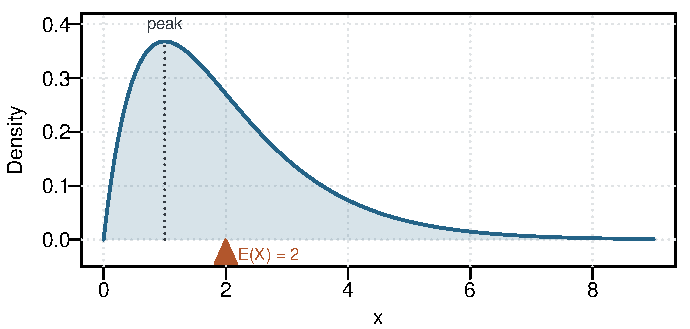
\includegraphics[width=.62\linewidth]{assets/rod-continuous.pdf}
\par\smallskip
{\footnotesize A density with a long right tail: $\mathbb{E}(X)$ lies to the right
of the peak.}
\end{center}

For a density with a long tail, $\mathbb{E}(X)$ does not lie under the peak
but is pulled towards the tail: to the right of the peak for a long right
tail, to the left for a long left tail. The tail carries little mass, but it is
far away and pushes hard, just like the weight $0.1$ at $10$ in
Example~\ref{ex:lottery-rod}. So $\mathbb{E}(X)$ is not the most likely value, which is the
peak, but the point where the distribution balances.

\begin{framedprop}{Symmetric distributions}\label{prop:symmetric}
Since $\mathbb{E}(X)$ is a centre of mass, if the distribution of $X$ is
symmetric about a point $x_0$ \emph{and} $\mathbb{E}(X)$ exists, then
$\mathbb{E}(X)=x_0$.
\end{framedprop}

The lever has a second, less pleasant consequence. A far-away weight pushes
hard even when it is light, so what happens to the balance point if we move
a tiny bit of probability very far from the origin?

\begin{framedprop}{Lack of robustness}\label{prop:robustness}
The expected value can be affected greatly by a very small change in the probability
assigned to a large value of $x$. Moving an amount $\varepsilon$ of
probability from a value $x_j$ to a point $M$ shifts $\mathbb{E}(X)$ by
$\varepsilon\,(M-x_j)$: however small $\varepsilon$ is, choosing $M$ far
enough moves $\mathbb{E}(X)$ arbitrarily far away.
\end{framedprop}

Why exactly $\varepsilon\,(M-x_j)$? In $\mathbb{E}(X)=\sum_x x\,p_X(x)$
only two terms change, while the probabilities still sum to $1$:
\begin{align*}
x_j\,p_X(x_j)&\;\longrightarrow\; x_j\,\big(p_X(x_j)-\varepsilon\big)
&&\text{loses } \varepsilon\,x_j,\\
M\,p_X(M)&\;\longrightarrow\; M\,\big(p_X(M)+\varepsilon\big)
&&\text{gains } \varepsilon\,M.
\end{align*}
The expected value therefore
changes by $\varepsilon\,M-\varepsilon\,x_j=\varepsilon\,(M-x_j)$.

\begin{center}
\begin{tabular}{@{}c@{\hspace{.04\linewidth}}c@{}}
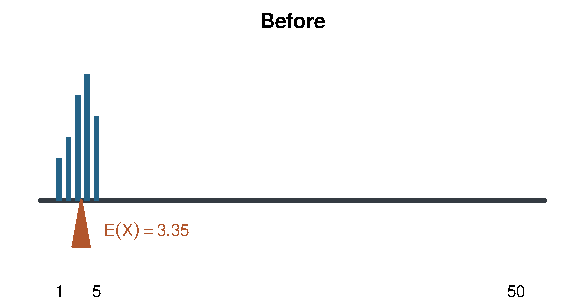
\includegraphics[width=.48\linewidth]{assets/far-before.pdf} &
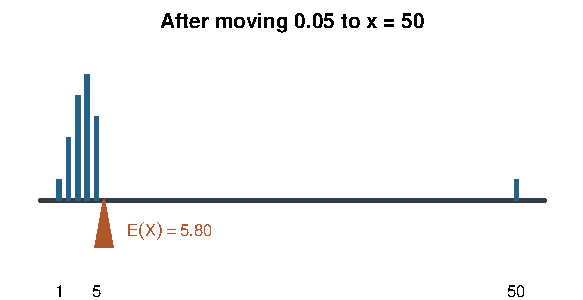
\includegraphics[width=.48\linewidth]{assets/far-after.pdf}\\
$\underbrace{\hspace{.46\linewidth}}_{\substack{
1(0.10)+2(0.15)+3(0.25)+4(0.30)+5(0.20)\\[2pt]
=\,3.35}}$ &
$\underbrace{\hspace{.46\linewidth}}_{\substack{
1(0.05)+2(0.15)+3(0.25)+4(0.30)+5(0.20)+50(0.05)\\[2pt]
=\,3.35+0.05\,(50-1)\,=\,5.80}}$
\end{tabular}
\end{center}


The expected value is therefore not robust to \emph{outliers}, rare values far from
the bulk of the distribution. When a model gives non-negligible probability
to values very far from the centre, as the distribution of the next section
does, other summaries such as the median can describe it better.

\section{Property 2: it may not exist}

The condition ``and $\mathbb{E}(X)$ exists'' in
Proposition~\ref{prop:symmetric} is not a formality. To see why, take a distribution that looks perfectly
well behaved: the Cauchy distribution
of Definition~\ref{def:cauchy}.

Recall that it is symmetric around $0$. So we would be tempted to say $\mathbb{E}(X)=0$.

Let us compute it. By definition,
\[
\mathbb{E}(X)=\int_{\mathbb{R}}\frac{x}{\pi\,(x^2+1)}\,\mathrm{d}x
=\frac{1}{2\pi}\int_{\mathbb{R}}\frac{2x}{x^2+1}\,\mathrm{d}x ,
\]
where we multiplied and divided by $2$ because $2x$ is the derivative of
$x^2+1$, so the integrand has the form $g'(x)/g(x)$ with $g(x)=x^2+1$, and a
primitive is $\log(x^2+1)$.

Recall that an integral over the whole real line is defined by splitting it at a point,
say $0$, and computing the two halves separately; it exists only when both
are finite, or at least do not diverge in opposite directions. Here
\[
\int_{0}^{+\infty}\frac{2x}{x^2+1}\,\mathrm{d}x
=\Big[\log(x^2+1)\Big]_{0}^{+\infty}=+\infty,
\qquad
\int_{-\infty}^{0}\frac{2x}{x^2+1}\,\mathrm{d}x
=\Big[\log(x^2+1)\Big]_{-\infty}^{0}=-\infty,
\]
and the total would be $-\infty+\infty$, which has no meaning. The
expected value of a Cauchy does not exist, symmetry notwithstanding.

The reason is in the tails. The integrand $x\,f_X(x)$ behaves like
$1/(\pi x)$ for large $|x|$: it goes to zero, but too slowly for its area
to be finite, while for the Normal it vanishes almost immediately.

\begin{center}
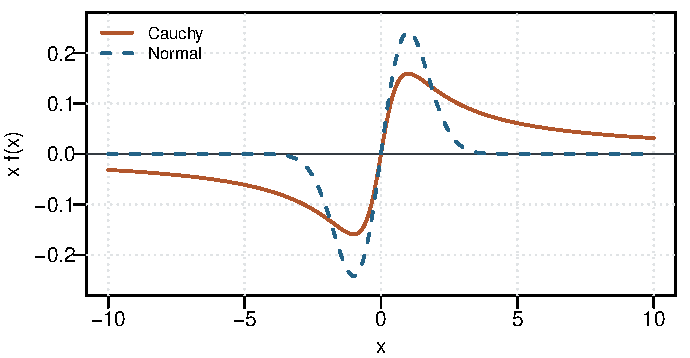
\includegraphics[width=.62\linewidth]{assets/cauchy-integrand.pdf}
\end{center}

This is exactly the situation that the condition in
Definition~\ref{def:expected-value} rules out. With $|x|$ in place of $x$
the two halves can no longer cancel: they add up, and here
\[
\int_{\mathbb{R}}|x|\,f_X(x)\,\mathrm{d}x
=\frac{1}{\pi}\int_{0}^{+\infty}\frac{2x}{x^2+1}\,\mathrm{d}x=+\infty ,
\]
so the condition fails and $\mathbb{E}(X)$ is not defined.

Yet the Cauchy clearly has a centre: it is symmetric around $0$ and peaks
there. If the expected value cannot describe it, what about the median?

\section{Property 3: the law of the lazy statistician}

Often we are not interested in $X$ itself but in a transformation of it:
its square $X^2$, its exponential $e^X$, a gain that depends on $X$.

Recall that we write $Y=r(X)$ for a \emph{deterministic} function $r$, that is a fixed
function with no randomness of its own: all the randomness of $Y$ comes
from $X$. How do we compute $\mathbb{E}(Y)$?

By definition, $\mathbb{E}(Y)$ is the weighted average of the values of
$Y$, so it needs the distribution of $Y$. Deriving it from the distribution
of $X$ is often long and inconvenient. The following theorem says we can
skip that step.

\begin{framedthm}{Law of the lazy statistician}\label{thm:lazy}
Let $X\sim F_X$ and $Y=r(X)$ for a deterministic function $r$. Then
\[
\mathbb{E}(Y)=\mathbb{E}\big(r(X)\big)=
\begin{cases}
\displaystyle\sum_x r(x)\,p_X(x) & \text{if $X$ is discrete,}\\[2ex]
\displaystyle\int_{\mathbb{R}} r(x)\,f_X(x)\,\mathrm{d}x & \text{if $X$ is continuous.}
\end{cases}
\]
\end{framedthm}

Only the distribution of $X$ is needed: each value $x$ is transformed into
$r(x)$ and weighted with the probability of $x$. That is why the statistician
is ``lazy''. Why is this true? In the discrete case
it is only a matter of reordering a sum.

\begin{proof}[Proof (discrete case)]
By definition, $\mathbb{E}(Y)=\sum_y y\,P(Y=y)$. The variable $Y$ takes the
value $y$ whenever $X$ takes any value $x$ with $r(x)=y$, so
\[
P(Y=y)=\sum_{x:\,r(x)=y}p_X(x).
\]
Substituting, and writing $y$ as $r(x)$ inside the inner sum, where
$r(x)=y$,
\[
\mathbb{E}(Y)=\sum_y\;\sum_{x:\,r(x)=y} r(x)\,p_X(x)=\sum_x r(x)\,p_X(x),
\]
because the double sum runs over every $x$ exactly once, grouped by the value
of $r(x)$.
\end{proof}

The continuous case follows the same idea, but needs more tools: for a
monotone differentiable $r$ it is a change of variables in the integral,
while for a general $r$ it requires measure theory.

\begin{framedexample}{The square of a die}\label{ex:die-square}
Let $X$ be the result of a fair die and $Y=X^2$. Without deriving the
distribution of $Y$,
\[
\mathbb{E}(X^2)=1^2\cdot\tfrac16+2^2\cdot\tfrac16+\cdots+6^2\cdot\tfrac16
=\frac{91}{6}\approx15.17 .
\]
\end{framedexample}

The law is everywhere, and it starts paying off at once. A first surprise:
probabilities themselves are expected values. Taking as $r$ the indicator function
$\mathbb{I}_A$ of an event $A$ gives the following result.

\begin{framedcor}{Probabilities are expected values}
For any event $A$,
\[
\mathbb{E}\big(\mathbb{I}_A(X)\big)=\int_{\mathbb{R}} \mathbb{I}_A(x)\,f_X(x)\,\mathrm{d}x
=\int_A f_X(x)\,\mathrm{d}x=P(X\in A).
\]
\end{framedcor}

As we mentioned before, the law also saves real work when the distribution
of $Y$ would be hard to find, as in the next example.

\begin{framedexample}{Transformation of a Unif$(0,1)$}
Let $X\sim\mathrm{Unif}(0,1)$, with $f_X(x)=1$ on $(0,1)$, and $Y=r(X)=e^X$.
Finding the density of $Y$ would require a change of variables, but the law
only needs $f_X$:
\[
\mathbb{E}(Y)\textcolor{NotesMuted}{\;\overset{\text{def}}{=}\;\int_{\mathbb{R}} y\,f_Y(y)\,\mathrm{d}y}=\int_0^1 e^x\cdot1\,\mathrm{d}x=\Big[e^x\Big]_0^1=e-1 .
\]
\end{framedexample}

Finally, the law computes moments, which by Definition~\ref{def:moments}
are expected values of powers of $X$.

\begin{framedexample}{Second moment of a Bernoulli}
Let $X\sim\mathrm{Ber}(p)$, so $X=1$ with probability $p$ and $X=0$ with
probability $1-p$. With $r(x)=x^2$,
\[
\mathbb{E}(X^2)=0^2\cdot(1-p)+1^2\cdot p=p .
\]
Since $0^2=0$ and $1^2=1$, here $X^2=X$, so the second moment equals the
first.
\end{framedexample}

\section{Property 4: Jensen inequality}

The law of the lazy statistician computes $\mathbb{E}\big(r(X)\big)$ by
transforming every value $x$ into $r(x)$ and then averaging. An even lazier
shortcut is tempting: average first, obtaining $\mathbb{E}(X)$, and transform
only that number, obtaining $r\big(\mathbb{E}(X)\big)$. Do the two agree?

In general they do not:
\[
\mathbb{E}\big(r(X)\big)\neq r\big(\mathbb{E}(X)\big).
\]

\begin{framedexample}{The square of a die, again}
Let us take the die of Example~\ref{ex:die-square} again, with
$r(x)=x^2$: there we found $\mathbb{E}(X^2)=91/6\approx15.17$, while
$\mathbb{E}(X)=3.5$. Squaring the average gives
\[
\big(\mathbb{E}(X)\big)^2=3.5^2=12.25\neq15.17\approx\mathbb{E}(X^2).
\]
\end{framedexample}

There is, however, a family of functions for which the two always agree.

\begin{framedprop}{Linear functions}\label{prop:linear}
If $r(x)=\alpha+\beta x$ for constants $\alpha$ and $\beta$, then
\[
\mathbb{E}\big(r(X)\big)=\mathbb{E}(\alpha+\beta X)=\alpha+\beta\,\mathbb{E}(X)
=r\big(\mathbb{E}(X)\big).
\]
\end{framedprop}

\begin{proof}[Proof (continuous case)]
By the law of the lazy statistician and the linearity of the integral,
\[
\mathbb{E}(\alpha+\beta X)=\int_{\mathbb{R}}(\alpha+\beta x)\,f_X(x)\,\mathrm{d}x
=\alpha\int_{\mathbb{R}}f_X(x)\,\mathrm{d}x+\beta\int_{\mathbb{R}}x\,f_X(x)\,\mathrm{d}x
=\alpha+\beta\,\mathbb{E}(X),
\]
since the density has total area $1$.
\end{proof}

The discrete case is the same, with sums in place of integrals.

\begin{framedexample}{Celsius and Fahrenheit}
A temperature $C$ in degrees Celsius becomes $F=32+1.8\,C$ in degrees
Fahrenheit. If $\mathbb{E}(C)=20$, then $\mathbb{E}(F)=32+1.8\cdot20=68$.
\end{framedexample}

The linearity of the integral only lets constants and sums out of it, so the
equality holds \emph{only} for linear functions: with $x^2$, $e^x$ or
$\log x$ nothing can be taken out.

For a non-linear $r$ the two quantities
\[
\mathbb{E}\big(r(X)\big)\qquad\text{and}\qquad r\big(\mathbb{E}(X)\big)
\]
are in general different. Is there still a general relationship between them?

For convex functions there is. Before stating it, let us see what convex
means.

\subsection{Convex functions}

Intuitively, a smooth function is convex when its graph always bends
upwards: it has a positive curvature at every point, like a bowl. For
functions with a second derivative, the curvature is exactly what the
second derivative measures.

\begin{framedprop}{Convexity and second derivative}
If $r$ is twice differentiable, then $r$ is convex on $S\subseteq\mathbb{R}$
if and only if $r''(x)\ge0$ for all $x\in S$.
\end{framedprop}

For example, $x^2$ is convex on $\mathbb{R}$, since its second derivative is
$2>0$, and so is $e^x$, whose second derivative is $e^x>0$.

The same idea has a geometric form that needs no derivatives: if we join
two points of the graph with a straight segment, the segment lies on or
above the graph. The points between $x_1$ and $x_2$ are written as
$t\,x_1+(1-t)\,x_2$ with $t\in[0,1]$, and at such a point the segment has
height $t\,r(x_1)+(1-t)\,r(x_2)$.

\begin{frameddefn}{Convex function}\label{def:convex}
A function $r:\mathbb{R}\to\mathbb{R}$ is \textbf{convex} on $S\subseteq\mathbb{R}$
if, for any $x_1,x_2\in S$ and $t\in[0,1]$,
\[
r\big(t\,x_1+(1-t)\,x_2\big)\le t\,r(x_1)+(1-t)\,r(x_2).
\]
It is \textbf{concave} if $-r$ is convex.
\end{frameddefn}

\begin{center}
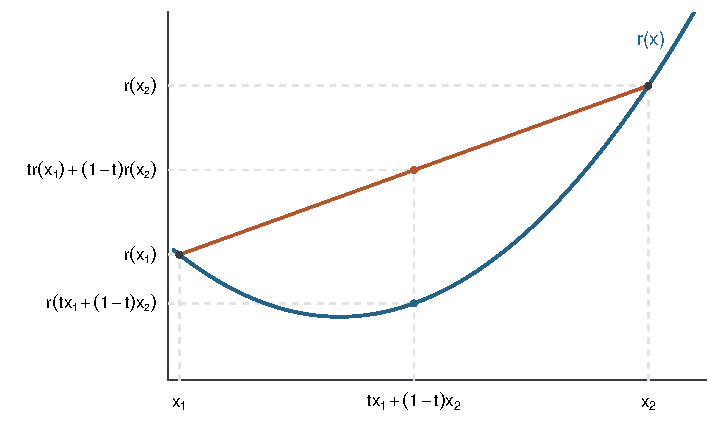
\includegraphics[width=.72\linewidth]{assets/convex-chord.pdf}
\end{center}

For a concave function the
segment lies below the graph and $r''(x)\le0$: for example $\log x$, whose
second derivative is $-1/x^2<0$.

\subsection{Jensen's inequality}

We can now answer the question for convex functions.

\begin{framedthm}{Jensen's inequality}\label{thm:jensen}
Let $X\sim F_X$ and let $r$ be a convex function, with $\mathbb{E}(X)$ and
$\mathbb{E}\big(r(X)\big)$ existing. Then
\[
r\big(\mathbb{E}(X)\big)\le\mathbb{E}\big(r(X)\big).
\]
If $r$ is concave, the inequality is reversed.
\end{framedthm}

Jensen's inequality is the definition of convexity rewritten in
probabilistic terms, as the case of a variable with two values shows.

\begin{proof}[Proof (two-valued case)]
Take $x_1,x_2$ and $t\in[0,1]$, and define a discrete random variable $X$
that takes two values,
\[
P(X=x_1)=t,\qquad P(X=x_2)=1-t .
\]
Its expected value is $\mathbb{E}(X)=t\,x_1+(1-t)\,x_2$, and by the law of
the lazy statistician
\[
\mathbb{E}\big(r(X)\big)=t\,r(x_1)+(1-t)\,r(x_2).
\]
Since $r$ is convex, Definition~\ref{def:convex} gives
\[
\underbrace{r\big(t\,x_1+(1-t)\,x_2\big)}_{r(\mathbb{E}(X))}
\;\le\;
\underbrace{t\,r(x_1)+(1-t)\,r(x_2)}_{\mathbb{E}(r(X))},
\]
which is exactly $r\big(\mathbb{E}(X)\big)\le\mathbb{E}\big(r(X)\big)$.
\end{proof}

We will see the proof for a general $X$ later.

Let us take the die of Example~\ref{ex:die-square} again: there
$r(x)=x^2$ is convex, and indeed
$\big(\mathbb{E}(X)\big)^2=12.25\le15.17\approx\mathbb{E}(X^2)$.

\begin{framedexample}{Arithmetic and geometric mean}
Since $\log x$ is concave, Jensen's inequality gives
$\log\mathbb{E}(X)\ge\mathbb{E}(\log X)$ for any positive random variable
$X$. Take data $x_1,\ldots,x_n>0$ and their empirical distribution, the
random variable $X$ with $P(X=x_i)=1/n$ for each $i$. Then
\[
\mathbb{E}(X)=\frac1n\sum_{i=1}^n x_i=\bar x_n,
\qquad
\mathbb{E}(\log X)=\frac1n\sum_{i=1}^n\log x_i=\log\Big(\prod_{i=1}^n x_i\Big)^{1/n},
\]
so Jensen's inequality reads
\[
\log\Big(\frac1n\sum_{i=1}^n x_i\Big)\ge\log\Big(\prod_{i=1}^n x_i\Big)^{1/n}
\quad\Longleftrightarrow\quad
\frac1n\sum_{i=1}^n x_i\ge\sqrt[n]{\prod_{i=1}^n x_i},
\]
where we exponentiated both sides, which keeps the inequality because $e^x$
is increasing. The arithmetic mean is always at least the geometric mean:
for $1$ and $4$, $2.5\ge\sqrt{4}=2$.
\end{framedexample}

\lecturestart[parts]{4 November}

Jensen's inequality also gives back Proposition~\ref{prop:linear}. What
happens if $r$ is both convex and concave? Then the segment between two
points of the graph lies both above and below the graph, so it lies exactly
on it:
\[
r\big(t\,x_1+(1-t)\,x_2\big)=t\,r(x_1)+(1-t)\,r(x_2).
\]
Every chord coincides with the graph, so the graph is a straight line.
With derivatives, $r''\ge0$ and $r''\le0$ give $r''=0$, that is
$r(x)=\alpha+\beta x$. Jensen's inequality now holds in both directions:
since $r$ is convex, $r\big(\mathbb{E}(X)\big)\le\mathbb{E}\big(r(X)\big)$,
and since $r$ is concave, $r\big(\mathbb{E}(X)\big)\ge\mathbb{E}\big(r(X)\big)$.
Together they give
\[
\mathbb{E}(\alpha+\beta X)=\alpha+\beta\,\mathbb{E}(X),
\]
which is Proposition~\ref{prop:linear} again.

The last example compares the expected value with the median. For
well-behaved random variables the two cannot be too far apart, and Jensen's
inequality tells us how far.

\begin{framedexample}{Expected value and median}
Let $\mu=\mathbb{E}(X)$, assuming it exists, and let $m$ be the median of
$X$. With the convex function $r(x)=|x|$,
\begin{align*}
|\mu-m|&=\big|\mathbb{E}(X)-m\big|=\big|\mathbb{E}(X-m)\big|
&&\text{linear functions}\\
&\le\mathbb{E}\,|X-m|&&\text{Jensen, $|x|$ convex}\\
&\le\mathbb{E}\,|X-\mu|&&\text{(}\heartsuit\text{)}\\
&=\mathbb{E}\sqrt{(X-\mu)^2}\\
&\le\sqrt{\mathbb{E}(X-\mu)^2}&&\text{Jensen, $\sqrt{x}$ concave.}
\end{align*}
Step $(\heartsuit)$ uses a property of the median that we will prove in
Property~5: among all constants $c$, the median minimises
$\mathbb{E}\,|X-c|$. The last quantity,
$\sigma=\sqrt{\mathbb{E}(X-\mu)^2}$, is the \textbf{standard deviation},
which we will meet again with the variance. Hence
\[
|\mu-m|\le\sigma :
\]
the expected value and the median are at most one standard deviation apart.
\end{framedexample}

\subsection{Jensen and the ELBO}

So far we have used Jensen's inequality to compare summaries of a
distribution. It also has an important use in \hyperref[alg:learning]{learning}, where it gives the
\textbf{evidence lower bound}, or \textbf{ELBO}. To see it, we need to talk a
little about learning again.

Recall from Section~\ref{sec:hidden} that we model what we observe together
with a hidden variable, through a joint distribution
$p(\text{obs},\text{hid})=p(\text{obs}\mid\text{hid})\,p(\text{hid})$, and
that the distribution of what we see is the mixture
\[
p(\text{obs})=\int_{\operatorname{supp}(\text{hid})} p(\text{obs},\text{hid})\,\mathrm{d}\,\text{hid}.
\]
Learning $\theta$ from the likelihood of such a mixture is hard: for a
\hyperref[def:gmm]{GMM} without labels there is no formula for $\hat\theta$,
which is problem~\spadeproblem. It would be easy if we knew the group of
every observation, since we could use
Proposition~\ref{prop:mle-gmm-labels}. But now we have learned Jensen's
inequality: could it help us solve problem~\spadeproblem?

The trouble is that we want to maximise the logarithm of an integral:
\[
\log p_\theta(\text{obs})=\log\int_{\operatorname{supp}(\text{hid})}
p_\theta(\text{obs},\text{hid})\,\mathrm{d}\,\text{hid}.
\]
The idea is to push back the hidden variable. Take any distribution $q$ over
the hidden variable, and multiply and divide by it inside the integral, which
changes nothing since $q/q=1$:
\[
\log p_\theta(\text{obs})=\log\int_{\operatorname{supp}(\text{hid})}
\underbrace{q(\text{hid})}_{\text{density}}\,
\underbrace{\frac{p_\theta(\text{obs},\text{hid})}{q(\text{hid})}}_{r(\text{hid})}\,
\mathrm{d}\,\text{hid}.
\]
By the \hyperref[thm:lazy]{law of the lazy statistician}:
\[
\log p_\theta(\text{obs})=\log\,\mathbb{E}_q\big(r(\text{hid})\big)
=\log\,\mathbb{E}_q\!\left[\frac{p_\theta(\text{obs},\text{hid})}{q(\text{hid})}\right].
\] We now have the logarithm of an
expected value, and $\log$ is concave: this is exactly the situation of
\hyperref[thm:jensen]{Jensen's inequality}.

By Jensen's inequality:
\[
\log p_\theta(\text{obs})=\log\,\mathbb{E}_q\!\left[\frac{p_\theta(\text{obs},\text{hid})}{q(\text{hid})}\right]
\;\ge\;\mathbb{E}_q\!\left[\log\frac{p_\theta(\text{obs},\text{hid})}{q(\text{hid})}\right]
=:F(q,\theta).
\]
What have we gained? On the left we still have the logarithm of a sum, the
one that blocked us in problem~\spadeproblem. On the right the logarithm has
moved inside the expected value, so we take the logarithm of each term
instead of the logarithm of their sum.

For a \hyperref[def:gmm]{GMM} the
terms are $\log\big(\pi_j\,N(o\mid\mu_j,\sigma_j^2)\big)$, which
split into simple pieces, as in the case with labels of
Proposition~\ref{prop:mle-gmm-labels}.

\begin{frameddefn}{ELBO}\label{def:elbo}
Let $\text{obs}$ be the observed variable, $\text{hid}$ the hidden one, and $q$ any
distribution of $\text{hid}$. The \textbf{evidence lower bound} (ELBO) is
\[
F(q,\theta)=\mathbb{E}_q\!\left[\log\frac{p_\theta(\text{obs},\text{hid})}{q(\text{hid})}\right].
\]
\emph{Evidence} refers to $\log p_\theta(\text{obs})$, the log-likelihood of what we
observe, and \emph{lower bound} to the fact that
$F(q,\theta)\le\log p_\theta(\text{obs})$ for every $q$ and every $\theta$.
\end{frameddefn}

The \hyperref[def:elbo]{ELBO} is our \textbf{surrogate target}: instead of maximising
$\log p_\theta(\text{obs})$, which is hard, as problem~\spadeproblem{} shows for a
\hyperref[def:gmm]{GMM}, we maximise $F(q,\theta)$, which is
easier. In the plot below the curve $F(q,\theta)$ never rises above
$\log p_\theta(\text{obs})$, so by pushing $F$ up we push up a lower bound of the
curve we care about.

\begin{center}
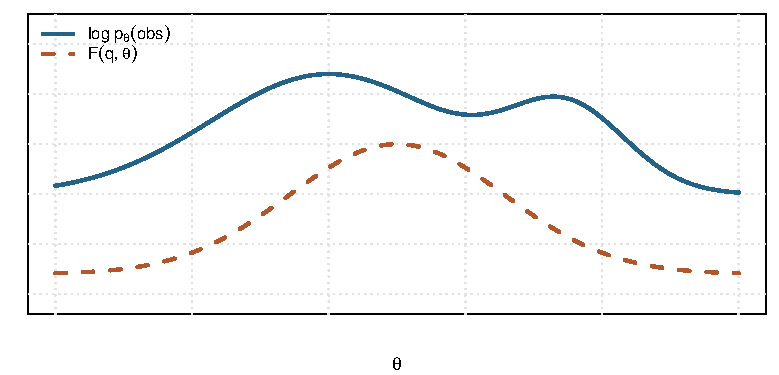
\includegraphics[width=.72\linewidth]{assets/elbo-sketch.pdf}
\end{center}

But does raising $F$ really raise $\log p_\theta(\text{obs})$ as well? Not
necessarily, as the next example shows.

% Keep the text and both plots of this example on one page.
\begingroup
\tcbset{examplebox/.append style={unbreakable}}
\begin{framedexample}{Raising $F$ while $\log p_\theta(\text{obs})$ goes down}\label{ex:elbo-before-after}
Keep $q$ fixed and take the two curves of the plot above. We start from
$\theta_{\text{old}}$, where $\log p_\theta(\text{obs})$ is close to its
highest point and $F(q,\theta)$ lies far below it. Then we move to
$\theta_{\text{new}}$, chosen so that $F$ goes up. In the plot on the
right the hollow points mark where we were: the orange point has risen, but
the blue one has gone down. Raising $F$ has lowered the log-likelihood.

\begin{center}
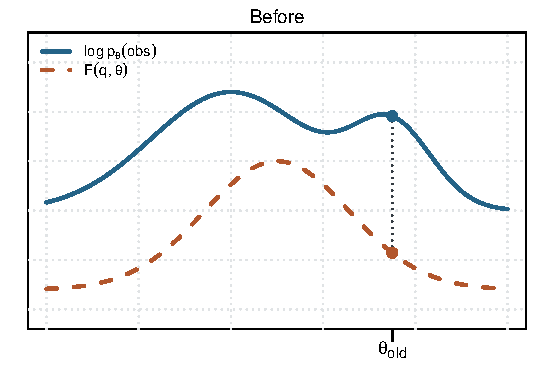
\includegraphics[width=.49\linewidth]{assets/elbo-before.pdf}\hfill
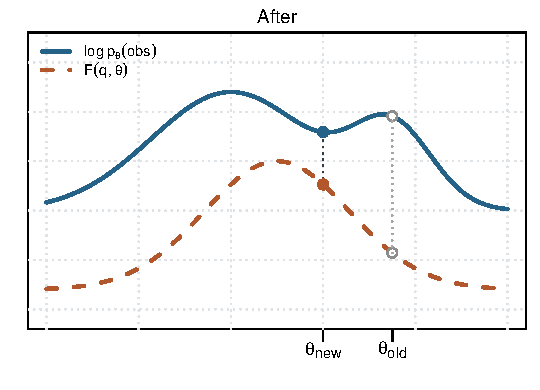
\includegraphics[width=.49\linewidth]{assets/elbo-after.pdf}
\end{center}
\end{framedexample}
\endgroup

Whether raising $F$ raises $\log p_\theta(\text{obs})$ depends on how wide
the gap between the two curves is: at $\theta_{\text{old}}$ the gap was so
wide that $F$ could rise a lot without telling us anything about
$\log p_\theta(\text{obs})$.

\lecturesecond{4 November}

\subsection{The information gap}\label{sec:information-gap}

How wide is the gap between the two curves? Let us give it a name and
compute it.

\begin{frameddefn}{Information gap}\label{def:information-gap}
The \textbf{information gap} is the difference between the log-likelihood and
the \hyperref[def:elbo]{ELBO},
\[
\log p_\theta(\text{obs})-F(q,\theta).
\]
\end{frameddefn}

By Jensen's inequality it is never negative. To see what it is, we write
$F$ as an integral and split the joint density with the multiplication
rule, $p_\theta(\text{obs},\text{hid})=p_\theta(\text{hid}\mid\text{obs})\,
p_\theta(\text{obs})$:
\begin{align*}
\log p_\theta(\text{obs})-F(q,\theta)
&=\log p_\theta(\text{obs})-\int q(\text{hid})\,
\log\frac{p_\theta(\text{obs},\text{hid})}{q(\text{hid})}\,\mathrm{d}\,\text{hid}\\
&=\log p_\theta(\text{obs})-\int q(\text{hid})\,
\log\frac{p_\theta(\text{hid}\mid\text{obs})\,p_\theta(\text{obs})}{q(\text{hid})}\,
\mathrm{d}\,\text{hid}.
\end{align*}
The logarithm of a product is the sum of the logarithms, so the integral
splits in two:
\[
=\log p_\theta(\text{obs})-\left[\int q(\text{hid})\,
\log\frac{p_\theta(\text{hid}\mid\text{obs})}{q(\text{hid})}\,\mathrm{d}\,\text{hid}
+\int q(\text{hid})\,\log p_\theta(\text{obs})\,\mathrm{d}\,\text{hid}\right].
\]
In the second integral $\log p_\theta(\text{obs})$ does not depend on
$\text{hid}$, so it comes out, and what is left integrates to $1$ because
$q$ is a distribution:
\[
\int q(\text{hid})\,\log p_\theta(\text{obs})\,\mathrm{d}\,\text{hid}
=\log p_\theta(\text{obs})\underbrace{\int q(\text{hid})\,\mathrm{d}\,\text{hid}}_{1}
=\log p_\theta(\text{obs}).
\]
The two copies of $\log p_\theta(\text{obs})$ cancel, and turning the
fraction upside down changes the sign of the logarithm:
\[
\log p_\theta(\text{obs})-F(q,\theta)
=\int q(\text{hid})\,\log\frac{q(\text{hid})}{p_\theta(\text{hid}\mid\text{obs})}\,
\mathrm{d}\,\text{hid}.
\]
This integral is a very specific way of measuring how far $q$ is from the
distribution of the hidden variable given what we observe.

\begin{frameddefn}{Kullback--Leibler divergence}\label{def:kl}
The \textbf{Kullback--Leibler divergence} (KL) of $q$ from $p$ is
\[
\mathrm{KL}(q\mid p)=\int q(x)\,\log\frac{q(x)}{p(x)}\,\mathrm{d}x.
\]
It is not a distance, and $\mathrm{KL}(q\mid p)=0$ if and only if $q=p$.
\end{frameddefn}

So the information gap is
\[
\log p_\theta(\text{obs})-F(q,\theta)
=\mathrm{KL}\big(q(\text{hid})\mid p_\theta(\text{hid}\mid\text{obs})\big),
\]
and it is zero exactly when
\[
q(\text{hid})=p_\theta(\text{hid}\mid\text{obs}).
\]
This answers our question: if we choose $q$ as the distribution of the
hidden variable given what we observe, the two curves touch, and
$F(q,\theta)=\log p_\theta(\text{obs})$ at that $\theta$.

In the plot below we take $\theta_{\text{old}}$ of
Example~\ref{ex:elbo-before-after} again and choose
$q=p_{\theta_{\text{old}}}(\text{hid}\mid\text{obs})$.

\begin{center}
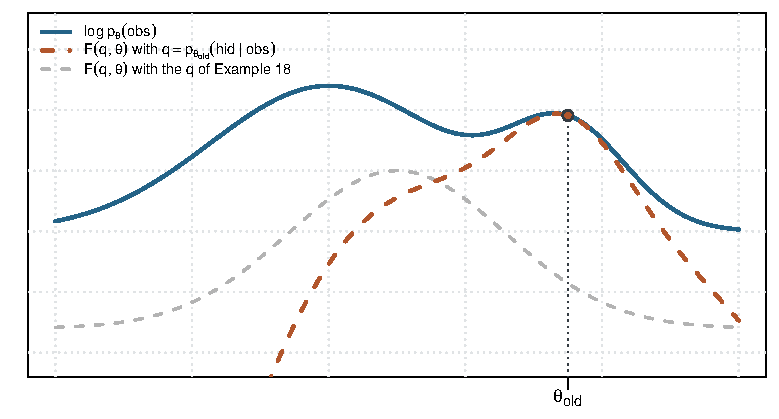
\includegraphics[width=.72\linewidth]{assets/elbo-touch.pdf}
\end{center}

How can we use this to climb $\log p_\theta(\text{obs})$?

\subsection{The EM algorithm}\label{sec:em}

The \hyperref[def:elbo]{ELBO} $F(q,\theta)$ depends on two things we can move: the distribution
$q$ and the parameter $\theta$. The typical way to use it is the
\textbf{EM algorithm}, one example of the wider family of MM algorithms.
The idea is \textbf{coordinate ascent} over $F(q,\theta)$: we move one
coordinate at a time, keeping the other fixed. First we optimise over $q$
with $\theta$ fixed, then over $\theta$ with $q$ fixed, and we repeat.

\begin{center}
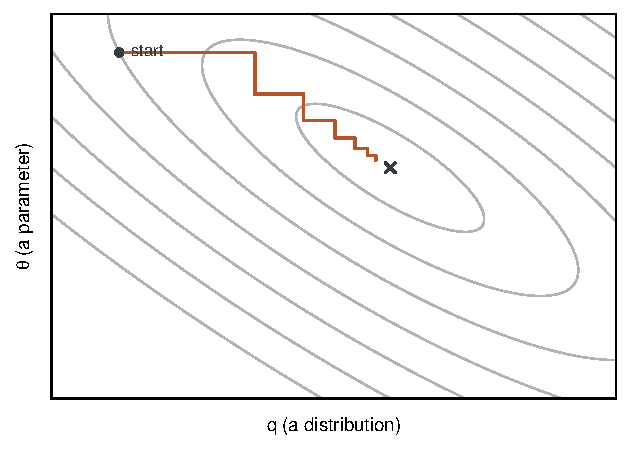
\includegraphics[width=.6\linewidth]{assets/em-coordinate-ascent.pdf}
\end{center}

In the plot each grey curve joins the points with the same value of $F$, and
the cross marks its maximum. A horizontal step changes only $q$, a vertical
step changes only $\theta$, and each step climbs as high as it can.

\begin{framedalgo}{EM algorithm}\label{alg:em}
Start from a parameter $\theta^{(0)}$. For $t=1,2,\ldots$ repeat:
\begin{enumerate}
\item \textbf{E-step.} Optimise over all distributions $q$, with $\theta$
fixed:
\[
q^{(t)}=\arg\max_{q}F\big(q,\theta^{(t-1)}\big).
\]
\item \textbf{M-step.} Optimise over all parameters $\theta$, with $q$
fixed:
\[
\theta^{(t)}=\arg\max_{\theta}F\big(q^{(t)},\theta\big).
\]
\end{enumerate}
\end{framedalgo}

\Needspace{5\baselineskip}\esteptag\par\smallskip
Which $q$ does the E-step choose? Recall from
Section~\ref{sec:information-gap} that
\[
F(q,\theta)=\log p_\theta(\text{obs})-\mathrm{KL}\big(q(\text{hid})\mid
p_\theta(\text{hid}\mid\text{obs})\big).
\]

With $\theta=\theta^{(t-1)}$ fixed,
the first term does not depend on $q$, so $F$ is largest when the
\hyperref[def:kl]{KL} is $0$, that is, when
\[
q^{(t)}(\text{hid})=p_{\theta^{(t-1)}}(\text{hid}\mid\text{obs}),
\]
if we can compute it.

\Needspace{5\baselineskip}\msteptag\par\smallskip
The M-step, instead, depends on the model: for a
\hyperref[def:gmm]{GMM} we will see it in the next lecture.

\vspace{\baselineskip}
Whatever form the M-step takes, does one round of EM really climb $\log p_\theta(\text{obs})$, the
target we want to maximise? Let us follow one round. At the beginning we are at
$\log p_{\theta^{(t-1)}}(\text{obs})$. Then:
\[
\log p_{\theta^{(t-1)}}(\text{obs})
\underbrace{=}_{\text{E-step}}F\big(q^{(t)},\theta^{(t-1)}\big)
\underbrace{\le}_{\text{M-step}}F\big(q^{(t)},\theta^{(t)}\big)
\underbrace{\le}_{\text{Jensen}}\log p_{\theta^{(t)}}(\text{obs}).
\]
\begin{itemize}
\item The E-step closes the gap, so $F$ equals the log-likelihood at
$\theta^{(t-1)}$: the two curves touch, as in the last plot.
\item The M-step chooses the $\theta$ with the largest $F$, so $F$ can only
go up.
\item By Jensen's inequality $F$ never rises above the log-likelihood.
\end{itemize}
So every round of EM increases, or at least does not decrease, the original
objective $\log p_\theta(\text{obs})$.

What does this look like round after round? In the sketch below we start
from $\theta^{(0)}$ and run two rounds of EM. In each E-step a new orange
curve touches the blue one at the current $\theta$; in each M-step we move to
the top of the orange curve, and the blue curve is higher there.

\begin{center}
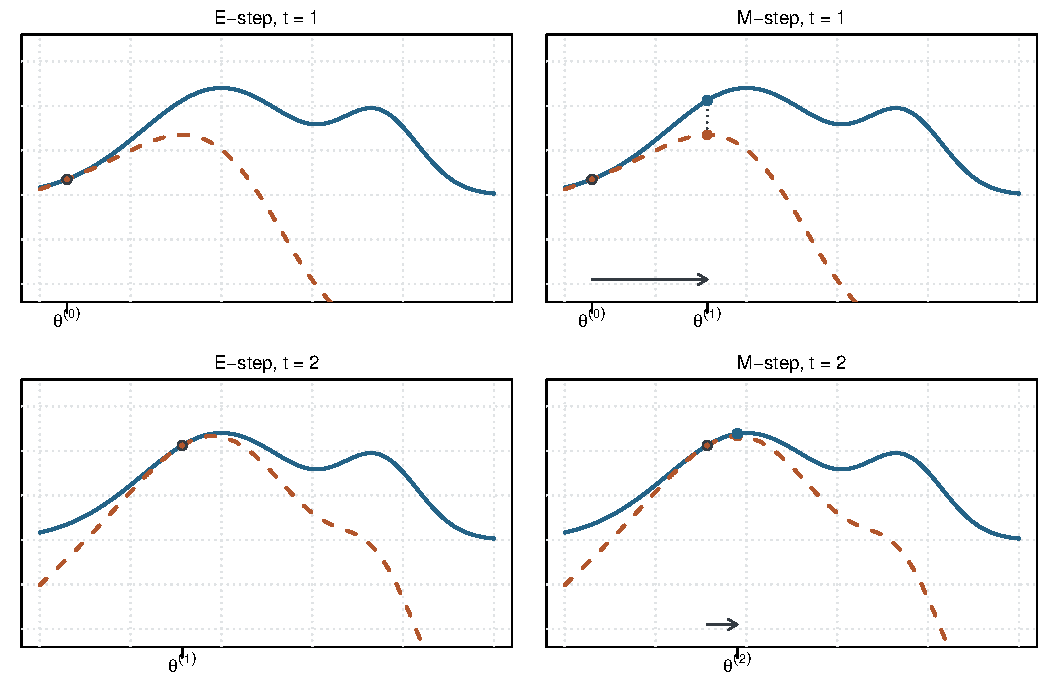
\includegraphics[width=\linewidth]{assets/em-steps.pdf}
\end{center}

The second step is shorter than the first: as EM approaches a maximum of
$\log p_\theta(\text{obs})$, each round gains less.

\paragraph{Remarks.} Both steps of Algorithm~\ref{alg:em} ask for a
maximum. Do we always get it, and do we really need it?
\begin{enumerate}
\item \textbf{E-step.} Optimising over \emph{all} distributions $q$ is
sometimes not feasible: sometimes $p_\theta(\text{hid}\mid\text{obs})$ is not
available. What do we do then? We optimise over a smaller class of
distributions instead of the whole class. This is the idea of
\textbf{variational methods}.
\item \textbf{M-step.} Here we are fine even without the exact maximum. In
the chain above the M-step is only used through
$F\big(q^{(t)},\theta^{(t-1)}\big)\le F\big(q^{(t)},\theta^{(t)}\big)$, so
any $\theta^{(t)}$ that does not lower $F$ still makes
$\log p_\theta(\text{obs})$ climb.
\end{enumerate}

\paragraph{What does the M-step maximise?} Let us split the \hyperref[def:elbo]{ELBO} in two. The
logarithm of a ratio is the difference of the logarithms, so
\[
F(q,\theta)
=\mathbb{E}_q\big[\log p_\theta(\text{obs},\text{hid})\big]
-\mathbb{E}_q\big[\log q(\text{hid})\big]
=\underbrace{\mathbb{E}_q\big[\log p_\theta(\text{obs},\text{hid})\big]}_{\text{expected complete log-likelihood}}
+\underbrace{H(q)}_{\text{entropy of }q},
\]
where $H(q)=-\mathbb{E}_q\big[\log q(\text{hid})\big]$ is called the
\textbf{entropy} of $q$. In the first term, $\log p_\theta(\text{obs},\text{hid})$ is the
\phantomsection\label{def:complete-loglik}\textbf{complete log-likelihood}, the one we would have if we also observed
the hidden variable, and we average it over $q$. The entropy
depends only on $q$, and in the M-step $q=q^{(t)}$ is fixed, so
\[
\theta^{(t)}=\arg\max_{\theta}F\big(q^{(t)},\theta\big)
=\arg\max_{\theta}\,\mathbb{E}_{q^{(t)}}\big[\log p_\theta(\text{obs},\text{hid})\big].
\]
The M-step maximises the expected complete log-likelihood: it works as if we
knew the hidden variable, weighting each of its values by $q^{(t)}$.

\lecturestart{5 November}

\subsection{EM for a Gaussian mixture}\label{sec:em-gmm}

So far we have presented the EM algorithm without going into the details,
in particular of the M-step.

Let us now run it on a concrete model: the
\hyperref[def:gmm]{GMM} without labels, the one of problem~\spadeproblem.
We have the data $o_1,\ldots,o_n$, a number of groups $K$ that we keep fixed,
and the likelihood
\[
L(\theta)=\prod_{i=1}^n\ \underbrace{\sum_{j=1}^K\pi_j\,
N(o_i\mid\mu_j,\sigma_j^2)}_{p_\theta(o_i)},
\qquad\theta=\{\pi_j,\mu_j,\sigma_j^2\}_{j=1}^K.
\]
What do the E-step and the M-step of Algorithm~\ref{alg:em} become here?

\Needspace{5\baselineskip}\esteptag\par\smallskip
As we saw in the \hyperref[sec:em]{EM algorithm}, the optimal choice is
$q(\text{hid})=p_\theta(\text{hid}\mid\text{obs})$, if we can compute it.
Let us see if we can. Each observation $o_i$ has its own hidden variable
$\text{hid}_i$, the group it comes from, and by Bayes' theorem its posterior
is
\[
p_\theta(\text{hid}_i=j\mid o_i)
=\frac{p_\theta(o_i\mid\text{hid}_i=j)\,p_\theta(\text{hid}_i=j)}{p_\theta(o_i)}
=\frac{\pi_j\,N(o_i\mid\mu_j,\sigma_j^2)}
{\sum_{k=1}^K\pi_k\,N(o_i\mid\mu_k,\sigma_k^2)}.
\]
Once $\theta$ is fixed every piece is
a number we can compute, and the denominator is a sum of only $K$ terms, so
for a GMM we can.

Notice that, since the denominator does not depend on $j$,
\[
p_\theta(\text{hid}_i=j\mid o_i)\propto p_\theta(o_i\mid\text{hid}_i=j)\,
p_\theta(\text{hid}_i=j).
\]

\begin{frameddefn}{Responsibilities}\label{def:responsibility}
The \textbf{responsibility} of group $j$ for the observation $o_i$ is the
posterior probability of its hidden variable,
\[
r_j^{(i)}=p_\theta(\text{hid}_i=j\mid o_i),
\qquad i=1,\ldots,n,\quad j=1,\ldots,K.
\]
\end{frameddefn}

\begin{framedexamplepart}{ex:men-women}{6}{Heights of men and women}
Let us take the heights of Example~\ref{ex:men-women} part~5 again. With the
labels we found $\hat\theta_{\text{women}}\approx(160.5,\,7.1^2)$,
$\hat\theta_{\text{men}}\approx(176.3,\,7.4^2)$ and weights
$\hat\pi_1=\hat\pi_2=0.5$. Suppose these are the current parameters of EM.
What responsibilities do the heights $147$, $167$ and $184$ get?

Using Bayes' theorem as above:
\begin{center}
\begin{tabular}{ccc}
\toprule
height $o_i$ & $r_{\text{women}}^{(i)}$ & $r_{\text{men}}^{(i)}$\\
\midrule
$147$ & $0.998$ & $0.002$\\
$167$ & $0.60$ & $0.40$\\
$184$ & $0.007$ & $0.993$\\
\bottomrule
\end{tabular}
\end{center}
A very short or very tall person is almost surely in one group. A height of
$167$~cm, between the two centres, is shared: $60\%$ women and $40\%$ men. Every
observation gets a weight for every group, instead of a single label.
\end{framedexamplepart}

\Needspace{5\baselineskip}\msteptag\par\smallskip
Once we have the responsibilities, the M-step looks for the new parameters
$\theta$. Recall that it maximises the
\hyperref[def:complete-loglik]{expected complete log-likelihood}:
\[
\theta^{(t)}=\arg\max_{\theta}\,\mathbb{E}_{q^{(t)}}\big[\log p_\theta(\text{obs},\text{hid})\big].
\]
Let us call the function to maximise
$E(\theta)=\mathbb{E}_{q^{(t)}}\big[\log p_\theta(\text{obs},\text{hid})\big]$.
For a GMM it is the double sum
\[
E(\theta)=\sum_{i=1}^n\sum_{j=1}^K r_j^{(i)}\,
\log\big(\pi_j\,N(o_i\mid\mu_j,\sigma_j^2)\big).
\]
The logarithm of a product is the sum of the logarithms, so
\[
E(\theta)=\sum_{i=1}^n\sum_{j=1}^K r_j^{(i)}\,
\Big[\log\pi_j+\log N(o_i\mid\mu_j,\sigma_j^2)\Big].
\]
Now we write the Normal density explicitly:
\[
E(\theta)=\sum_{i=1}^n\sum_{j=1}^K r_j^{(i)}\,
\Big[\log\pi_j+\log\Big(\frac{1}{\sqrt{2\pi}\,\sigma_j}\,
\exp\Big(-\frac{(o_i-\mu_j)^2}{2\sigma_j^2}\Big)\Big)\Big].
\]
The second logarithm is again the logarithm of a product, so it is the sum
of the logarithms of its three factors:
\[
E(\theta)=\sum_{i=1}^n\sum_{j=1}^K r_j^{(i)}\,
\Big[\log\pi_j+\log\frac{1}{\sqrt{2\pi}}+\log\frac{1}{\sigma_j}
+\log\exp\Big(-\frac{(o_i-\mu_j)^2}{2\sigma_j^2}\Big)\Big].
\]
Since $\log\frac1a=-\log a$, $\log\sqrt{a}=\tfrac12\log a$ and the logarithm
cancels the exponential,
\[
E(\theta)=\sum_{i=1}^n\sum_{j=1}^K r_j^{(i)}\,
\Big[\log\pi_j-\tfrac12\log(2\pi)-\log\sigma_j
-\frac{(o_i-\mu_j)^2}{2\sigma_j^2}\Big].
\]
The term $-\tfrac12\log(2\pi)$ does not depend on $\theta$, so it does not
change where the maximum is, and we can drop it:
\[
E(\theta)=\sum_{i=1}^n\sum_{j=1}^K r_j^{(i)}\Big[\log\pi_j-\log\sigma_j
-\frac{(o_i-\mu_j)^2}{2\sigma_j^2}\Big]+\text{const}.
\]

At the start we could not maximise the likelihood with a closed form,
because of the logarithm of a sum in problem~\spadeproblem. Now the
logarithm is inside the sums, and each term is as simple as in the case
with labels. So now we can.

\paragraph{The centres.} Only the terms of group $j$ contain $\mu_j$. Setting
the derivative to zero,
\[
\frac{\partial E}{\partial\mu_j}=\sum_{i=1}^n r_j^{(i)}\,
\frac{o_i-\mu_j}{\sigma_j^2}=0
\quad\Longleftrightarrow\quad
\hat\mu_j=\frac{\sum_{i=1}^n r_j^{(i)}\,o_i}{\sum_{i=1}^n r_j^{(i)}}.
\]
The new centre of group $j$ is a weighted average of the observations: each
one counts as much as its responsibility for group $j$.

\paragraph{The spreads.} In the same way, setting to zero the derivative
with respect to $\sigma_j$,
\[
\frac{\partial E}{\partial\sigma_j}=\sum_{i=1}^n r_j^{(i)}
\Big[-\frac{1}{\sigma_j}+\frac{(o_i-\mu_j)^2}{\sigma_j^3}\Big]=0
\quad\Longleftrightarrow\quad
\hat\sigma_j^2=\frac{\sum_{i=1}^n r_j^{(i)}\,(o_i-\hat\mu_j)^2}
{\sum_{i=1}^n r_j^{(i)}}.
\]
The new $\hat\sigma_j^2$ is a weighted average of the squared distances from
the new centre.

Compare these with \hyperref[prop:mle-gmm-labels]{maximum likelihood for a
GMM with labels}. If each responsibility were $1$ for the true group and $0$
for the others, $\sum_i r_j^{(i)}$ would be $n_j$, and $\hat\mu_j$ and
$\hat\sigma_j^2$ would be the centre and the spread computed from the
observations of group $j$ only. The M-step is maximum likelihood with labels, where the
labels $0$ or $1$ are replaced by the responsibilities.

\begin{framedexamplepart}{ex:men-women}{7}{Heights of men and women}
Let us take the three heights of Example~\ref{ex:men-women} part~6 again:
$147$, $167$ and $184$, with responsibilities $0.998$, $0.60$ and $0.007$
for women and $0.002$, $0.40$ and $0.993$ for men. If these three were all
our data, where would the M-step move the two centres?

For women,
\[
\hat\mu_{\text{women}}
=\frac{0.998\cdot147+0.60\cdot167+0.007\cdot184}{0.998+0.60+0.007}
\approx\frac{248.2}{1.605}\approx154.6,
\]
and in the same way $\hat\mu_{\text{men}}\approx179.1$. The height $147$ pulls
the women's centre almost with its full weight, $167$ pulls it with weight
$0.60$, and $184$ hardly at all.
\end{framedexamplepart}

\paragraph{The weights.} The weights are different: they must be
non-negative and add up to $1$, so they lie in the
\hyperref[def:simplex]{simplex}. Maximising $E(\theta)$ over the weights is
therefore an optimisation with a constraint, which is solved with Lagrange
multipliers, a tool we will see later. The result is
\[
\hat\pi_j=\frac{\sum_{i=1}^n r_j^{(i)}}{n},
\]
the share of the observations that group $j$ is responsible for. With
labels $0$ or $1$ it becomes $n_j/n$, as in the case with labels.

\paragraph{Putting it together.} One round of EM for a GMM is:
\begin{enumerate}
\item \textbf{E-step:} with the current parameters, compute the
responsibilities $r_j^{(i)}$ of every group for every observation;
\item \textbf{M-step:} with these responsibilities, compute the new centres
$\hat\mu_j$, spreads $\hat\sigma_j^2$ and weights $\hat\pi_j$.
\end{enumerate}
We repeat the two steps, and by the check of
Section~\ref{sec:em} the log-likelihood never goes down. This is the
tool that problem~\spadeproblem\ was waiting for: without labels there is
still no single formula for $\hat\theta$, but we can now fit a GMM by
climbing its likelihood one round at a time.

\end{document}
